\chapter{Metode Penelitian}

\section{Metode yang Digunakan}

Metode yang digunakan adalah \textit{prototyping} dengan tahapan perancangan,
implementasi, dan pengujian. Evaluasi utama memverifikasi kontrol terpilih
melalui skenario fungsional dan kebijakan \textit{endorsement}, serta mengukur
kapasitas lokal tiga \textit{chaincode} eksperimen pada jaringan empat MSP
menggunakan Hyperledger Caliper.
Siklus SDLC metode \textit{prototyping} yang diterapkan ditunjukkan
pada Gambar~\ref{fig:sdlc-proto}: keempat fase (analisis kebutuhan, perancangan,
implementasi, dan evaluasi) diulang secara iteratif hingga purwarupa memenuhi
spesifikasi.

% Siklus SDLC metode prototyping (TikZ).
% Di-input dari BAB III §3.1.2.1.

\begin{figure}[H]
\centering
\resizebox{0.72\textwidth}{!}{%
\begin{tikzpicture}[
  phase/.style={draw=black, fill=white, rectangle, rounded corners=4pt,
    minimum width=3.2cm, minimum height=1.0cm, align=center, font=\footnotesize\bfseries},
  center/.style={draw=none, fill=none, align=center, font=\small\itshape},
  ar/.style={-{Stealth}, very thick},
]

%--- Empat fase membentuk lingkaran ---
%  0°=kanan, 90°=atas  →  posisi fase:
%  Atas: Analisis Kebutuhan
%  Kanan: Perancangan
%  Bawah: Implementasi
%  Kiri: Evaluasi

\node[phase] (req)   at ( 0,  3.4) {Analisis\\Kebutuhan};
\node[phase] (design) at ( 3.4, 0) {Perancangan\\Purwarupa};
\node[phase] (impl)  at ( 0, -3.4) {Implementasi};
\node[phase] (eval)  at (-3.4, 0) {Evaluasi \&\\Pengujian};

\node[center] at (0, 0) {Siklus\\\textit{Prototyping}};

%--- Panah siklus (searah jarum jam) ---
\draw[ar] (req.east)   to[bend left=25]  (design.north);
\draw[ar] (design.south) to[bend left=25] (impl.east);
\draw[ar] (impl.west)  to[bend left=25]  (eval.south);
\draw[ar] (eval.north) to[bend left=25]  (req.west);

%--- Label panah ---
\node[font=\scriptsize, align=center] at ( 2.8,  2.4) {rancang\\\textit{prototype}};
\node[font=\scriptsize, align=center] at ( 2.8, -2.4) {bangun\\\textit{prototype}};
\node[font=\scriptsize, align=center] at (-2.8, -2.4) {uji \&\\evaluasi};
\node[font=\scriptsize, align=center] at (-2.8,  2.4) {perbaiki\\kebutuhan};

\end{tikzpicture}%
}
\caption{Siklus SDLC dengan metode \textit{prototyping}: empat fase berulang hingga purwarupa memenuhi kebutuhan fungsional dan kinerja}
\label{fig:sdlc-proto}
\end{figure}


\subsection{Metode Perancangan}

Perancangan sistem dimulai dari analisis kebutuhan berdasarkan model Rupiah
Digital dua jenjang, kemudian dituangkan ke dalam activity diagram, arsitektur
sistem, arsitektur jaringan, perancangan use case, dan model data
\textit{ledger}.

\subsubsection{Analisis Kebutuhan Sistem}

Analisis kebutuhan mengidentifikasi aktor sistem (Bank Indonesia, bank
validator, PJP, pedagang, pelanggan ritel, supervisor, dan pengamat OJK) beserta
kebutuhan fungsionalnya, yaitu penerbitan dan distribusi likuiditas berjenjang,
transfer antarpelanggan serta pelanggan-ke-pedagang, pengawasan, dan pelaporan.
Kebutuhan ini menjadi dasar perancangan activity diagram dan arsitektur
pada subbab berikutnya.

\subsubsection{Spesifikasi Kebutuhan Perangkat Lunak}

Analisis kebutuhan tersebut diformalkan dalam bentuk Spesifikasi Kebutuhan
Perangkat Lunak (\textit{Software Requirements Specification}/SRS) yang diadaptasi
ke struktur tesis ini. SRS digunakan untuk menetapkan ruang lingkup purwarupa,
aktor dan batas wewenangnya, antarmuka utama sistem, kebutuhan fungsional, dan
kebutuhan nonfungsional sebelum implementasi dilakukan. Pada penelitian ini,
ruang lingkup perangkat lunak mencakup empat antarmuka utama, yaitu aplikasi
klien, \textit{backend API}, basis data luring PostgreSQL, dan jaringan
\textit{blockchain} Hyperledger Fabric beserta \textit{chaincode}-nya. Aplikasi klien hanya berfungsi sebagai alat bantu demonstrasi dan tidak termasuk dalam evaluasi penelitian ini.

Pemangku kepentingan utama terdiri atas Bank Indonesia sebagai penerbit dan
pengawas, bank distributor dan PJP sebagai kustodian institusional, pedagang dan
pelanggan ritel sebagai pengguna transaksi, serta supervisor dan pengamat OJK
sebagai pihak yang membutuhkan fungsi baca dan pelaporan. Setiap pemangku
kepentingan tersebut kemudian diterjemahkan menjadi
peran akses pada \textit{backend API} dan aturan bisnis pada \textit{chaincode}
agar kebutuhan operasional dapat ditelusuri secara konsisten.

\begin{table}[H]
    \caption{Kebutuhan fungsional purwarupa bi-coin}
    \label{tab:srs-fungsional}
    \centering
    \small
    \begin{tabular}{@{}p{1.5cm}p{9.8cm}@{}}
        \toprule
        \textbf{ID} & \textbf{Deskripsi kebutuhan} \\
        \midrule
        FR-01 & Sistem harus mendukung pendaftaran, persetujuan, pembekuan, pencairan, dan penghentian peserta sesuai peran Bank Indonesia, bank distributor, dan PJP. \\
        FR-02 & Sistem harus mendukung penerbitan Digital Rupiah oleh Bank Indonesia ke dalam Treasury dan distribusi langsung kepada bank distributor atau PJP sebagai kustodian institusional. \\
        FR-03 & Sistem harus menolak transfer yang tidak diotorisasi, melibatkan dompet beku, bernilai tidak valid, atau melebihi saldo pengirim, lalu memperbarui saldo secara atomik. \\
        FR-04 & Sistem harus menyediakan laporan rekonsiliasi, metrik, riwayat transaksi, dan \textit{event} pengawasan bagi peran yang berwenang. \\
        FR-05 & Sistem harus menegakkan pemisahan hak akses pada \textit{backend API} antara peran publik, terautentikasi, PJP/bank, merchant, dan supervisor. \\
        \bottomrule
    \end{tabular}
\end{table}

\begin{table}[H]
    \caption{Kebutuhan nonfungsional purwarupa bi-coin}
    \label{tab:srs-nonfungsional}
    \centering
    \small
    \begin{tabular}{@{}p{1.7cm}p{9.6cm}@{}}
        \toprule
        \textbf{ID} & \textbf{Deskripsi kebutuhan} \\
        \midrule
        NFR-01 & Sistem harus berjalan pada jaringan \textit{permissioned} Hyperledger Fabric yang mendukung partisipasi multipihak dan kebijakan \textit{endorsement} organisasi yang ditetapkan pada kanal. \\
        NFR-02 & Sistem harus menyediakan keterlacakan melalui catatan audit, \textit{event} pengawasan, dan riwayat transaksi yang dapat ditelusuri kembali ke peserta terkait. \\
        NFR-03 & Sistem harus memisahkan antarmuka klien, \textit{backend API}, basis data luring, dan \textit{chaincode} agar kontrol akses dan integrasi dapat dikelola secara modular. \\
        NFR-04 & Sistem harus dapat dievaluasi kinerjanya secara kuantitatif melalui metrik \textit{throughput}, latensi, dan tingkat keberhasilan transaksi menggunakan Hyperledger Caliper. \\
        NFR-05 & Sistem harus mendukung pengulangan eksperimen pada lingkungan yang sama melalui konfigurasi, \textit{seed}, hash artefak, topologi jaringan, dan skenario uji yang terdokumentasi. \\
        \bottomrule
    \end{tabular}
\end{table}

\begin{table}[H]
    \caption{Keterlacakan kebutuhan terhadap metode verifikasi}
    \label{tab:srs-verifikasi}
    \centering
    \small
    \begin{tabular}{@{}p{1.8cm}p{4.7cm}p{4.8cm}@{}}
        \toprule
        \textbf{ID kebutuhan} & \textbf{Metode verifikasi utama} & \textbf{Bukti yang dituju} \\
        \midrule
        FR-01, FR-02 & Skenario fungsional dan \textit{unit test} \textit{chaincode} & Siklus hidup peserta, penerbitan, dan distribusi dua jenjang berjalan sesuai aturan \\
        FR-03 & \textit{Unit test} \textit{backend} dan \textit{chaincode} serta skenario transfer & Otorisasi, status beku, validasi saldo, dan pembaruan atomik ditegakkan konsisten \\
        FR-04, FR-05 & Skenario fungsional, \textit{unit test} \textit{backend}, dan inspeksi rute API & Hak akses, pelaporan, dan \textit{event} pengawasan tersedia bagi peran berwenang \\
        NFR-01, NFR-03, NFR-05 & Inspeksi arsitektur, konfigurasi, dan manifes benchmark & Struktur jaringan, pemisahan lapisan, dan \textit{repeatability} purwarupa terdokumentasi \\
        NFR-02 & Inspeksi model data dan \textit{unit test} terpilih & Keterlacakan audit dan riwayat transaksi dapat dipertahankan \\
        NFR-04 & \textit{Benchmark} Hyperledger Caliper & Nilai \textit{throughput}, latensi, dan tingkat keberhasilan transaksi diperoleh secara kuantitatif \\
        \bottomrule
    \end{tabular}
\end{table}

\subsubsection{Perancangan Activity Diagram}

Setiap proses utama dimodelkan dengan activity diagram bergaya
\textit{swimlane} tiga jalur, yaitu jalur aktor, jalur \textit{backend API}, dan
jalur \textit{blockchain} (\textit{chaincode}). Diagram tersebut mencakup
pendaftaran peserta (Gambar~\ref{fig:ad01}), penerbitan Digital Rupiah
(Gambar~\ref{fig:ad02}), distribusi likuiditas dari Treasury Bank Indonesia kepada kustodian
(Gambar~\ref{fig:ad03}). Proses lainnya meliputi transfer saldo ritel
(Gambar~\ref{fig:ad05}), pembekuan dan pencairan peserta
(Gambar~\ref{fig:ad08}), serta laporan dan pengawasan
(Gambar~\ref{fig:ad10}).

% Activity diagram sistem Rupiah Digital.
% Keenam gambar di-render dari blok bernama pada berkas PlantUML:
%   bi-coin-fabric/docs/diagrams/plantuml/activity-diagrams.puml
% Untuk merender:
%   cd /path/to/bi-coin && rtk python render-activity-diagrams.py
% Di-input dari BAB III §3.2.4.

\newcommand{\actfig}[3]{%
  \begin{figure}[H]\centering
  \IfFileExists{contents/figures/activity/#1.png}{%
    \includegraphics[width=\textwidth,height=0.78\textheight,keepaspectratio]%
      {contents/figures/activity/#1.png}%
  }{%
    \fbox{\parbox{0.9\textwidth}{\centering\small
      \textit{[Gambar belum di-render. Jalankan:
      \texttt{rtk python render-activity-diagrams.py}]}\\
      \texttt{#1.png}}}%
  }%
  \caption{#2}
  \label{#3}
  \end{figure}
}

\newcommand{\actfiglandscape}[3]{%
  \begin{figure}[H]\centering
  \IfFileExists{contents/figures/activity/#1.png}{%
    \rotatebox{90}{\includegraphics[width=0.72\textheight]%
      {contents/figures/activity/#1.png}}%
  }{%
    \fbox{\parbox{0.9\textwidth}{\centering\small
      \textit{[Gambar belum di-render. Jalankan:
      \texttt{rtk python render-activity-diagrams.py}]}\\
      \texttt{#1.png}}}%
  }%
  \caption{#2}
  \label{#3}
  \end{figure}
}

\actfiglandscape{AD01-Pendaftaran-Peserta}%
  {Activity diagram pendaftaran peserta}{fig:ad01}

\actfig{AD02-Penerbitan-Digital-Rupiah}%
  {Activity diagram penerbitan w-Rupiah Digital langsung ke reserve Distributor Bank}{fig:ad02}

\actfig{AD03-Transfer-Konversi-Pendanaan}%
  {Activity diagram transfer antarbank, konversi, dan pendanaan dompet}{fig:ad03}

\actfig{AD05-Transfer-Saldo-Ritel}%
  {Activity diagram transfer saldo ritel}{fig:ad05}


\actfig{AD08-Pembekuan-Peserta}%
  {Activity diagram pembatasan dan pembukaan pembatasan peserta oleh staf Distributor (Compliance Officer, KYC Reviewer, Senior Approver)}{fig:ad08}

\actfiglandscape{AD10-Laporan-Supervisi}%
  {Activity diagram pembacaan status subjek oleh Auditor}{fig:ad10}


\subsubsection{Perancangan Arsitektur Sistem Blockchain}

Arsitektur pada subbab ini menjelaskan jaringan studi empat organisasi yang
digunakan untuk pengukuran kinerja dan pengujian kontrol, yaitu
\texttt{CentralBankMSP}, \texttt{DistributorMSP}, \texttt{ValidatorMSP}, dan
\texttt{EndUserMSP}. Rincian lingkungan studi kontrol dijelaskan pada bagian
eksperimen kontrol di bawah.

Secara konseptual, sistem menggunakan model distribusi Rupiah Digital dua
jenjang sebagaimana ditunjukkan pada Gambar~\ref{fig:arsitektur-dua-jenjang}.
Jenjang distribusi institusional menyalurkan Digital Rupiah dari Treasury Bank
Indonesia selaku penerbit (\texttt{CentralBankMSP}) kepada bank dan PJP sebagai
kustodian institusional (\texttt{DistributorMSP}) melalui jaringan Hyperledger
Fabric. Jenjang layanan ritel menyediakan pembayaran melalui kustodian kepada
pengguna ritel, pedagang, dan pengguna bisnis (\texttt{EndUserMSP}), termasuk
transfer antarpelanggan,
transfer pelanggan-ke-pedagang, dan kontrol akses berbasis peran. Jenjang
institusional tersebut menjelaskan jalur distribusi menuju layanan ritel, bukan
implementasi instrumen w-Digital
Rupiah yang terpisah.

% Arsitektur dua jenjang sistem Rupiah Digital (TikZ), purwarupa empat organisasi.
% Di-input dari BAB III §3.2.1 sebelum fig:arsitektur.

\begin{figure}[H]
\centering
\resizebox{\textwidth}{!}{%
\begin{tikzpicture}[
  actor/.style={draw=black, fill=white, rectangle, rounded corners=3pt,
    minimum width=3.2cm, minimum height=1.0cm, align=center, font=\footnotesize\bfseries},
  wbox/.style={draw=black, fill=gray!10, rectangle, rounded corners=2pt,
    minimum width=3.0cm, minimum height=0.9cm, align=center, font=\scriptsize},
  zonebox/.style={draw=black, dashed, rounded corners=6pt, fill=none, inner sep=14pt},
  pl/.style={font=\scriptsize, midway, align=center},
  ar/.style={-{Stealth}, thick},
  dar/.style={-{Stealth}, thick, dashed},
]

%── Jenjang distribusi institusional ──────────────────────────────────────────

\node[actor] (bi)          at (0,    0)    {Bank Indonesia\\(Penerbit)\\CentralBankMSP};
\node[actor] (distributor) at (7.0,  0)    {Distributor\\(bank dan PJP)\\DistributorMSP};
\node[actor] (validator)   at (14.0, 0)    {Validator\\(OJK, PPATK)\\ValidatorMSP, observer};

% BI Treasury → Distributor (penerbitan dan distribusi)
\draw[ar] (bi.east) -- node[pl, above]{Distribusi dari Treasury} (distributor.west);

% Pelaporan dan akses baca pengawasan
\draw[dar] (distributor.east) -- node[pl, above]{Laporan} (validator.west);
\draw[dar] (bi.north) to[out=60,in=120] node[pl, above]{Akses baca} (validator.north);

\node[zonebox,
  fit=(bi)(distributor)(validator),
  label={[font=\footnotesize\bfseries, anchor=north west]south west:%
    Jenjang 1: Distribusi Institusional}] (j1) {};

%── Batas jenjang ─────────────────────────────────────────────────────────────

\draw[dashed, thick, gray!70] (-1.0, -2.8) -- (15.5, -2.8);
\node[font=\scriptsize, gray!70, anchor=east] at (15.5, -2.55)
  {Batas jenjang distribusi};

%── Distribusi lintas jenjang ─────────────────────────────────────────────────

\node[actor] (enduser) at (7.0, -4.5) {EndUser\\(EndUserMSP)};

\draw[ar] (distributor.south) -- node[pl, right]{Distribusi langsung\\ke EndUser} (enduser.north);

%── Jenjang 2: Retail ────────────────────────────────────────────────────────

\node[wbox] (customer) at (3.5,  -6.8) {Pelanggan Ritel};
\node[wbox] (merchant) at (7.0,  -6.8) {Pedagang};
\node[wbox] (business) at (10.5, -6.8) {Bisnis};

\draw[ar] (enduser.south) -- (customer.north);
\draw[ar] (enduser.south) -- (merchant.north);
\draw[ar] (enduser.south) -- (business.north);

\node[zonebox,
  fit=(enduser)(customer)(merchant)(business),
  label={[font=\footnotesize\bfseries, anchor=south west]north west:%
    Jenjang 2: Layanan Ritel}] (j2) {};

\node[font=\scriptsize, gray] at (7.0, -8.3)
  {Transfer P2P/pedagang};

\end{tikzpicture}%
}
\caption{Arsitektur distribusi dua jenjang pada purwarupa Rupiah Digital ritel dengan empat organisasi: Bank Indonesia (CentralBankMSP) menerbitkan, Distributor (bank dan PJP) mendistribusikan, EndUser (ritel, pedagang, dan bisnis) melayani, dan Validator (OJK, PPATK) mengawasi secara baca.}
\label{fig:arsitektur-dua-jenjang}
\end{figure}


Arsitektur teknologi Rupiah Digital dalam White Paper CBDC Bank Indonesia
terdiri atas lapisan platform teknologi, lapisan aset digital, dan lapisan use
case. Komponen dasarnya mencakup \textit{sandbox}, API, \textit{smart contract},
layanan identitas, layanan regulasi, dan pengamanan kriptografi sebagaimana
ditunjukkan pada Gambar~\ref{fig:bi-whitepaper-technology-architecture}
\cite{bi_whitepaper2022}. Purwarupa \textit{bi-coin-fabric} memetakan gagasan
tersebut secara terbatas melalui API backend, \textit{chaincode}, identitas
organisasi, peran pengawasan, serta \textit{ledger} Hyperledger Fabric. Pemetaan
terbatas ini menjadikan purwarupa sebagai model eksperimental yang selaras
dengan prinsip arsitektur BI, bukan representasi penuh arsitektur produksi
Rupiah Digital.

\begin{figure}[H]
    \centering
    \rotatebox{90}{\includegraphics[width=0.78\textheight]{contents/figures/reference/bi-whitepaper-technology-architecture.png}}
    \caption{Arsitektur teknologi Rupiah Digital menurut White Paper CBDC Bank Indonesia. Sumber: Bank Indonesia \cite{bi_whitepaper2022}.}
    \label{fig:bi-whitepaper-technology-architecture}
\end{figure}

Sistem dirancang sebagai arsitektur layanan \textit{backend API} dan jaringan
\textit{blockchain} sebagaimana ditunjukkan pada Gambar~\ref{fig:arsitektur}.
Lapisan \textit{backend API} bertindak sebagai \textit{gateway} yang
menerjemahkan permintaan HTTP menjadi pemanggilan \textit{chaincode} sekaligus
menegakkan kontrol akses berbasis peran, sedangkan lapisan jaringan
\textit{blockchain} menjalankan \textit{chaincode} serta menyimpan
\textit{ledger}.

Kontrol akses memakai dua batas kepercayaan. Backend memvalidasi JWT, membatasi
rute menurut peran, mencatat subjek dan peserta pemanggil, lalu memilih gateway
Fabric berdasarkan MSP kustodian pada konteks permintaan. Untuk pengguna ritel,
backend juga mencocokkan subjek JWT dengan \texttt{owner\_id} dompet pengirim.
Chaincode memvalidasi MSP pemanggil dan MSP kustodian dompet: mutasi moneter,
dan siklus hidup peserta hanya menerima MSP yang diizinkan, sedangkan
MSP pengamat tidak dapat memutasi buku besar. Kepemilikan nasabah tetap menjadi
batas kepercayaan backend karena identitas pemilik tidak digantikan oleh
identitas klien Fabric pada chaincode.

Berdasarkan klasifikasi model pembayaran pada Bab~2, purwarupa
\textit{bi-coin-fabric} dikategorikan sebagai model dompet ritel berbasis akun
(\textit{account-based wallet model}) yang diimplementasikan di atas
\textit{ledger} Hyperledger Fabric. Klasifikasi ini diturunkan dari rancangan
data \textit{on-chain}: objek \texttt{Wallet} menyimpan \texttt{OwnerID},
status beku, dan \texttt{Balance}; fungsi \texttt{Transfer} memeriksa
otorisasi, status beku, dan saldo, kemudian mendebit saldo pengirim
serta mengkredit saldo penerima. Sistem tidak membentuk objek token pembawa
(\textit{bearer token}), UTXO, atau nomor seri token yang berpindah antarpemilik.
Mekanisme pembayaran purwarupa berupa dompet berbasis akun yang disederhanakan,
bukan model token murni. Model tersebut digunakan untuk menguji transfer ritel
dan auditabilitas transaksi.

% Arsitektur sistem penuh Rupiah Digital: client → backend → Fabric → peers
% Purwarupa studi empat organisasi (kanal bi-coin)
% Di-input dari BAB III §3.1.3

\begin{figure}[H]
\centering
\resizebox{\textwidth}{!}{%
\begin{tikzpicture}[
  appbox/.style={draw=black, fill=white, rectangle, rounded corners=3pt,
    minimum width=5.0cm, minimum height=1.1cm, align=center, font=\small},
  gwbox/.style={draw=black, fill=black!5, rectangle, rounded corners=3pt,
    minimum width=5.0cm, minimum height=1.1cm, align=center, font=\small},
  pgbox/.style={draw=black, fill=blue!8, rectangle, rounded corners=3pt,
    minimum width=3.8cm, minimum height=1.1cm, align=center, font=\small},
  peer/.style={draw=black, fill=white, rectangle, rounded corners=2pt,
    minimum width=3.2cm, minimum height=1.1cm, align=center, font=\scriptsize},
  obsbox/.style={draw=black, dashed, fill=white, rectangle, rounded corners=2pt,
    minimum width=3.2cm, minimum height=1.1cm, align=center, font=\scriptsize},
  ordnode/.style={draw=black, fill=black!8, rectangle, rounded corners=3pt,
    minimum width=3.8cm, minimum height=1.1cm, align=center, font=\scriptsize\bfseries},
  cdb/.style={draw=black, fill=gray!20, rectangle,
    minimum width=2.5cm, minimum height=0.75cm, align=center, font=\scriptsize},
  cabox/.style={draw=black, fill=yellow!20, rectangle, rounded corners=2pt,
    minimum width=2.5cm, minimum height=0.75cm, align=center, font=\tiny},
  ar/.style={-{Stealth}, thick},
  bar/.style={{Stealth}-{Stealth}, thick},
  lbl/.style={font=\scriptsize, midway},
]

%── Lapisan Aplikasi ──────────────────────────────────────────────────────────

\node[appbox] (fe) at (6.0, 16.5) {\textbf{Client}\\Web UI / Client App};
\node[appbox] (be) at (6.0, 14.5) {\textbf{Backend API}\\Go REST + Gorilla Mux + JWT/RBAC};
\node[pgbox]  (pg) at (0.0, 14.5) {\textbf{PostgreSQL}\\Portal authentication};
\node[gwbox]  (gw) at (6.0, 12.5) {\textbf{Fabric Gateway SDK v1.8}\\gRPC / TLS};

\draw[ar]  (fe.south) -- (be.north)  node[lbl, right]{HTTP/REST};
\draw[bar] (be.west)  -- (pg.east)   node[lbl, above]{SQL};
\draw[ar]  (be.south) -- (gw.north)  node[lbl, right]{Gateway API};

%── Jaringan Hyperledger Fabric ───────────────────────────────────────────────
% Latar belakang kotak digambar PERTAMA agar node internal tampak di atasnya

\fill[rounded corners=8pt, gray!5]  (-2.8, 2.2) rectangle (12.8, 11.0);
\draw[rounded corners=8pt, black]   (-2.8, 2.2) rectangle (12.8, 11.0);
\node[font=\scriptsize\bfseries, anchor=north west, align=left] at (-2.5, 10.8)
  {\textbf{Hyperledger Fabric 2.5}\\
   kanal \textit{bi-coin}, kontrak \textit{rupiah-monetary}, \textit{rupiah-controls}, \textit{rupiah-payments}, kebijakan endorsement per kontrak, TLS};

% Panah dari Gateway ke batas atas kotak jaringan
\draw[ar] (gw.south) -- (6.0, 11.0)
  node[lbl, right]{\textit{endorse} + submit (gRPC)};

%── Orderer ───────────────────────────────────────────────────────────────────

\node[ordnode] (ord) at (5.25, 9.5)
  {orderer.centralbank.bi-coin:7050\\Raft (satu node)};

%── Empat Peer ────────────────────────────────────────────────────────────────

\node[peer]   (pcb)   at (0.0, 7.0)
  {peer0.centralbank.bi-coin\\CentralBankMSP\\:17051};
\node[peer]   (pdist) at (3.5, 7.0)
  {peer0.distributor.bi-coin\\DistributorMSP\\:18051};
\node[obsbox] (pval)  at (7.0, 7.0)
  {peer0.validator.bi-coin\\ValidatorMSP (observer)\\:19051};
\node[peer]   (pusr)  at (10.5, 7.0)
  {peer0.enduser.bi-coin\\EndUserMSP\\:20051};

% Orderer → semua peer (pengiriman blok)
\draw[ar] (ord.south) to[out=-110,in=80] (pcb.north);
\draw[ar] (ord.south) to[out=-100,in=80] (pdist.north);
\draw[ar] (ord.south) to[out=-80,in=100]  (pval.north);
\draw[ar] (ord.south) to[out=-70,in=100]  (pusr.north);

%── CouchDB (satu per organisasi) ─────────────────────────────────────────────

\node[cdb] (ccb)   at (0.0,  5.5) {CouchDB :17584};
\node[cdb] (cdist) at (3.5,  5.5) {CouchDB :18584};
\node[cdb] (cval)  at (7.0,  5.5) {CouchDB :19584};
\node[cdb] (cusr)  at (10.5,  5.5) {CouchDB :20584};

\draw[ar] (pcb)   -- (ccb);
\draw[ar] (pdist) -- (cdist);
\draw[ar] (pval)  -- (cval);
\draw[ar] (pusr)  -- (cusr);

%── Empat CA, satu per organisasi (di bawah kotak jaringan) ───────────────────

\node[cabox] (ca1) at (0.0, 1.0)
  {CA ca.centralbank.bi-coin\\(CentralBankMSP)};
\node[cabox] (ca2) at (3.5, 1.0)
  {CA ca.distributor.bi-coin\\(DistributorMSP)};
\node[cabox] (ca3) at (7.0, 1.0)
  {CA ca.validator.bi-coin\\(ValidatorMSP)};
\node[cabox] (ca4) at (10.5, 1.0)
  {CA ca.enduser.bi-coin\\(EndUserMSP)};
\draw[ar] (ca1.north) -- (0.0, 2.2);
\draw[ar] (ca2.north) -- (3.5, 2.2);
\draw[ar] (ca3.north) -- (7.0, 2.2);
\draw[ar] (ca4.north) -- (10.5, 2.2);

\end{tikzpicture}%
}
\caption{Arsitektur purwarupa studi Rupiah Digital: lapisan \textit{client}, \textit{backend API} (Go REST + JWT/RBAC), basis data PostgreSQL luring, \textit{Fabric Gateway SDK}, serta jaringan Hyperledger Fabric 2.5 dengan empat organisasi (CentralBankMSP, DistributorMSP, ValidatorMSP, EndUserMSP), satu CouchDB per organisasi, empat CA (satu per organisasi), dan orderer Raft satu node}
\label{fig:arsitektur}
\end{figure}


Jaringan studi \textit{blockchain} dirancang dengan empat organisasi, yaitu
\texttt{CentralBankMSP}, \texttt{DistributorMSP}, \texttt{ValidatorMSP}, dan
\texttt{EndUserMSP}. Setiap organisasi memiliki satu \textit{peer} dan satu basis
data status CouchDB. Keempat organisasi tersebut merepresentasikan peran Bank
Indonesia, bank dan PJP, pengawas, serta pengguna akhir pada model dua jenjang.
\textit{Orderer} Raft dengan satu node (\texttt{orderer.centralbank.rupiah.study})
dan satu CA (\texttt{ca.centralbank}) diselenggarakan oleh \texttt{CentralBankMSP},
dengan batas waktu pemotongan blok dua detik dan maksimum sepuluh
\textit{message} per blok. Rincian organisasi disajikan pada
Tabel~\ref{tab:jaringan}.

\begingroup
\renewcommand{\arraystretch}{1.3}
\begin{table}[H]
	\caption{Organisasi pada jaringan studi Rupiah Digital}
	\label{tab:jaringan}
	\centering
	\small
	\begin{tabular}{p{2.9cm} p{2.7cm} p{3.4cm} p{3.4cm}}
	\toprule
	\textbf{Organisasi} & \textbf{Peran} & \textbf{Peran pada jaringan} & \textbf{MSP} \\
	\midrule
	Bank Indonesia & Penerbit dan pengawas & Penerbitan dan penarikan Digital Rupiah; menyelenggarakan \textit{orderer} dan CA tunggal & \texttt{CentralBankMSP} \\
	Bank dan PJP & Distributor & Kustodian institusional penerima distribusi dari Bank Indonesia; wajib dalam kebijakan \textit{endorsement} default ketiga \textit{chaincode} & \texttt{DistributorMSP} \\
	OJK, PPATK, dan supervisor & \textit{Validator} & Akses baca untuk audit dan pengawasan; tidak termasuk dalam kebijakan \textit{endorsement} default & \texttt{ValidatorMSP} \\
	Pedagang, pelanggan ritel, dan pengguna bisnis & Pengguna & Pelaku transaksi ritel; ikut memberikan \textit{endorsement} pada pembayaran bersama \texttt{DistributorMSP} & \texttt{EndUserMSP} \\
	\bottomrule
	\end{tabular}
\end{table}
\endgroup

Seluruh peserta tergabung dalam satu kanal (\textit{channel}) \texttt{rupiah-study}.
Kebijakan \textit{endorsement} dan siklus hidup \textit{chaincode} default pada
kanal menggunakan \texttt{MAJORITY Endorsement}, sedangkan tiga \textit{chaincode}
eksperimen memiliki kebijakan \textit{endorsement} tersendiri sebagaimana
dirangkum pada bagian eksperimen kontrol di bawah.
Komunikasi antarsimpul diamankan dengan TLS.
Topologi jaringan secara lengkap ditunjukkan pada
Gambar~\ref{fig:arsitektur-jaringan}, yang memperlihatkan hubungan antara
\textit{orderer}, keempat \textit{peer}, basis data CouchDB masing-masing
organisasi, serta \textit{backend API} yang terhubung ke jaringan melalui
\textit{Fabric Gateway SDK}.

% Arsitektur jaringan Hyperledger Fabric sistem Rupiah Digital (TikZ).
% Purwarupa studi empat organisasi, kanal bi-coin.
% Di-input dari BAB III §3.2.2 setelah tab:jaringan.

\begin{figure}[H]
\centering
\resizebox{\textwidth}{!}{%
\begin{tikzpicture}[
  peer/.style={draw=black, fill=white, rectangle, rounded corners=2pt,
    minimum width=3.2cm, minimum height=0.9cm, align=center, font=\scriptsize},
  observer/.style={draw=black, dashed, fill=none, rectangle, rounded corners=2pt,
    minimum width=3.2cm, minimum height=0.9cm, align=center, font=\scriptsize},
  cdb/.style={draw=black, fill=gray!12, rectangle,
    minimum width=2.2cm, minimum height=0.6cm, align=center, font=\scriptsize},
  ordnode/.style={draw=black, fill=black!8, rectangle, rounded corners=3pt,
    minimum width=3.4cm, minimum height=0.9cm, align=center, font=\footnotesize\bfseries},
  backend/.style={draw=black, fill=black!5, rectangle, rounded corners=3pt,
    minimum width=4.0cm, minimum height=0.9cm, align=center, font=\footnotesize},
  chanbox/.style={draw=black, dashed, rounded corners=5pt,
    fill=none, inner sep=8pt},
  ar/.style={-{Stealth}, thick},
  gar/.style={-{Stealth}, thick, dashed},
  pathlabel/.style={font=\scriptsize, midway, align=center},
]

%--- Backend + Orderer ---
\node[backend] (be)  at (-2.5, 3.5) {Backend API\\Go + Fabric Gateway SDK};
\node[ordnode] (ord) at ( 5.25, 3.5) {orderer.centralbank.bi-coin:7050\\(Raft, satu node)};
\draw[ar] (be.east) -- node[pathlabel,above]{gRPC} (ord.west);

%--- Peer nodes (empat organisasi) ---
\node[peer]     (pcb)   at ( 0.0, 1.2) {peer0.centralbank.bi-coin\\CentralBankMSP\\:17051};
\node[peer]     (pdist) at ( 3.5, 1.2) {peer0.distributor.bi-coin\\DistributorMSP\\:18051};
\node[observer] (pval)  at ( 7.0, 1.2) {peer0.validator.bi-coin\\ValidatorMSP (observer)\\:19051};
\node[peer]     (pusr)  at (10.5, 1.2) {peer0.enduser.bi-coin\\EndUserMSP\\:20051};

%--- Orderer delivers block to all peers ---
\draw[ar] (ord.south) to[out=-100,in=90] (pcb.north);
\draw[ar] (ord.south) to[out=-100,in=90] (pdist.north);
\draw[ar] (ord.south) -- (pval.north);
\draw[ar] (ord.south) to[out=-80,in=90]  (pusr.north);

%--- Backend gateway ke peer0.distributor (gateway peer contoh pada network/README.md) ---
\draw[gar] (be.south) -- node[pathlabel,above,sloped]{\textit{endorse}} (pdist.north);

%--- CouchDB state databases (satu per organisasi) ---
\node[cdb] (ccb)   at ( 0.0, -0.2) {CouchDB :17584};
\node[cdb] (cdist) at ( 3.5, -0.2) {CouchDB :18584};
\node[cdb] (cval)  at ( 7.0, -0.2) {CouchDB :19584};
\node[cdb] (cusr)  at (10.5, -0.2) {CouchDB :20584};

\draw[ar] (pcb)   -- (ccb);
\draw[ar] (pdist) -- (cdist);
\draw[ar] (pval)  -- (cval);
\draw[ar] (pusr)  -- (cusr);

%--- bi-coin bounding box ---
\node[chanbox, fit=(pcb)(pdist)(pval)(pusr)(ccb)(cdist)(cval)(cusr),
  label={[font=\footnotesize\bfseries]below:%
    \textit{bi-coin} (kebijakan endorsement per kontrak, TLS)}] {};

\end{tikzpicture}%
}
\caption{Arsitektur jaringan purwarupa studi Rupiah Digital pada kanal \texttt{bi-coin} dengan empat organisasi}
\label{fig:arsitektur-jaringan}
\end{figure}


Kebutuhan fungsional sistem dimodelkan dengan diagram use case. Aktor sistem
terdiri atas Bank Indonesia, bank distributor, PJP, pedagang (\textit{merchant}),
pelanggan ritel, supervisor, dan pengamat OJK. Diagram use case keseluruhan
ditunjukkan pada Gambar~\ref{fig:uc01}, sedangkan rincian operasi
institusional dan ritel ditunjukkan pada Gambar~\ref{fig:uc02} dan
Gambar~\ref{fig:uc03}.

% Diagram use case sistem Rupiah Digital (TikZ).
% Di-input dari BAB III.

\tikzset{
  uactor/.style={draw=none, fill=none, minimum width=0.9cm,
    minimum height=1.3cm, inner sep=0pt},
  ucase/.style={draw=black, fill=white, ellipse, minimum width=3.2cm,
    minimum height=0.95cm, inner sep=2pt, align=center, font=\scriptsize},
  ubox/.style={draw=black, dashed, fill=none, rectangle},
  udep/.style={draw=black, dashed, -{Stealth}, font=\scriptsize},
  uassoc/.style={draw=black, -{Stealth}},
}

% UML stick-figure actor: #1=node id, #2=(x,y) position, #3=label
\newcommand{\umlactor}[3]{%
  \node[uactor] (#1) at #2 {};%
  \begin{scope}[shift={#2}]
    \draw[thick] (0,0.30) circle (0.13);          % kepala
    \draw[thick] (0,0.17) -- (0,-0.18);           % badan
    \draw[thick] (-0.22,0.02) -- (0.22,0.02);     % lengan
    \draw[thick] (0,-0.18) -- (-0.18,-0.5);       % kaki kiri
    \draw[thick] (0,-0.18) -- (0.18,-0.5);        % kaki kanan
  \end{scope}
  \node[font=\scriptsize, align=center, anchor=north] at ($#2+(0,-0.58)$) {#3};%
}

\begin{figure}[H]
\centering
\resizebox{\textwidth}{!}{%
\begin{tikzpicture}
\umlactor{bi}{(0,8)}{Bank\\Indonesia}
\umlactor{dist}{(0,6)}{Distributor\\(bank dan PJP)}
\umlactor{m}{(12,8)}{Merchant}
\umlactor{pr}{(12,6)}{Pelanggan\\Ritel}
\umlactor{sv}{(12,4)}{Supervisor}
\umlactor{val}{(12,2)}{Validator\\(OJK, PPATK)}

\node[ubox, minimum width=8cm, minimum height=8.5cm] (sys) at (6,5) {};
\node[font=\footnotesize\bfseries] at (6,9.6) {Sistem Rupiah Digital (bi-coin-fabric)};

\node[ucase] (uc1) at (6,9) {Mendaftarkan Peserta};
\node[ucase] (uc2) at (6,8) {Menerbitkan Digital Rupiah};
\node[ucase] (uc3) at (6,7) {Mendistribusikan Likuiditas\\ke Peserta};
\node[ucase] (uc5) at (6,5) {Mentransfer Saldo};
\node[ucase] (uc6) at (6,4) {Transfer ke Pedagang};
\node[ucase] (uc7) at (6,2.8) {Bekukan/Cairkan Peserta};
\node[ucase] (uc9) at (6,0.4) {Laporan \& Pengawasan};

\draw[uassoc] (bi) -- (uc1);
\draw[uassoc] (dist) to[out=70,in=188] (uc1.west);
\draw[uassoc] (bi) -- (uc2);
\draw[uassoc] (bi) -- (uc3);
\draw[uassoc] (bi) -- (uc7);
\draw[uassoc] (bi) -- (uc3);
\draw[uassoc] (m) -- (uc6);
\draw[uassoc] (pr) -- (uc5);
\draw[uassoc] (pr) -- (uc6);
\draw[uassoc] (sv) -- (uc9);
\draw[uassoc] (bi) to[out=-95,in=172] (uc9.west);
\draw[uassoc, dashed] (val) -- (uc9) node[midway, above, sloped, font=\scriptsize]{$\langle\langle$observasi$\rangle\rangle$};
\end{tikzpicture}%
}
\caption{Diagram use case keseluruhan sistem Rupiah Digital}
\label{fig:uc01}
\end{figure}

\begin{figure}[H]
\centering
\resizebox{0.92\textwidth}{!}{%
\begin{tikzpicture}
\umlactor{bi}{(0,6)}{Bank\\Indonesia}
\umlactor{dist}{(0,3.5)}{Distributor\\(bank dan PJP)}
\umlactor{sv}{(10,3.5)}{Supervisor}

\node[ubox, minimum width=6cm, minimum height=6.5cm] (sys) at (5,3.5) {};
\node[font=\footnotesize\bfseries] at (5,7.2) {Operasi Institusional};

\node[ucase] (w1) at (5,6) {Menerbitkan dan Menebus\\Digital Rupiah};
\node[ucase] (w2) at (5,5) {Mendistribusikan Likuiditas\\ke Peserta};
\node[ucase] (w3) at (5,4) {Mengelola Siklus Hidup\\Peserta};
\node[ucase] (w5) at (5,2) {Mengajukan Pendaftaran\\Peserta};
\node[ucase] (w6) at (5,1) {Membaca Laporan \& Metrik};

\draw[uassoc] (bi) -- (w1);
\draw[uassoc] (bi) -- (w2);
\draw[uassoc] (bi) -- (w3);
\draw[uassoc] (bi) -- (w5);
\draw[uassoc] (bi) -- (w6);
\draw[uassoc] (bi) -- (w2);
\draw[uassoc] (dist) -- (w5);
\draw[uassoc] (sv) -- (w6);
\end{tikzpicture}%
}
\caption{Diagram use case operasi institusional}
\label{fig:uc02}
\end{figure}

\begin{figure}[H]
\centering
\resizebox{0.92\textwidth}{!}{%
\begin{tikzpicture}
\umlactor{pr}{(0,6)}{Pelanggan\\Ritel}
\umlactor{m}{(10,6)}{Merchant}

\node[ubox, minimum width=6cm, minimum height=5.5cm] (sys) at (5,4) {};
\node[font=\footnotesize\bfseries] at (5,7.2) {Operasi Retail};

\node[ucase] (r2) at (5,4.7) {Transfer Antarpelanggan};
\node[ucase] (r3) at (5,3.4) {Transfer ke Pedagang};
\draw[uassoc] (pr) -- (r2);
\draw[uassoc] (pr) -- (r3);
\draw[uassoc] (m) -- (r3);
\end{tikzpicture}%
}
\caption{Diagram use case operasi retail}
\label{fig:uc03}
\end{figure}


Pemetaan aktor pada diagram tersebut mengikuti kendali peran pada lapisan
\textit{backend}. Pendaftaran peserta dapat diajukan oleh institusi, sedangkan
persetujuan, penolakan, pembekuan, dan \textit{offboarding} hanya dapat
dilakukan oleh Bank Indonesia. Supervisor dan pengamat OJK hanya memperoleh
jalur baca pengawasan. Status persetujuan peserta menjadi bagian dari siklus
hidup peserta, bukan bukti alur persetujuan terpisah.

Status sistem disimpan pada \textit{world state} dalam bentuk objek-objek yang
dirangkum pada Tabel~\ref{tab:model-data}. Objek-objek ini menjadi dasar seluruh
operasi \textit{chaincode}.

\begingroup
\renewcommand{\arraystretch}{1.3}
\begin{longtable}{>{\RaggedRight\arraybackslash}p{4.4cm}
                  >{\RaggedRight\arraybackslash}p{8.5cm}}
	\caption{Objek status utama pada ledger}\label{tab:model-data}                        \\
	\toprule
	\textbf{Objek}             & \textbf{Keterangan}                                      \\
	\midrule
	\endfirsthead
	\toprule
	\textbf{Objek}             & \textbf{Keterangan}                                      \\
	\midrule
	\endhead
	\bottomrule
	\endlastfoot
	\texttt{Participant}       & Entitas peserta (validator/observer/PJP), MSP kustodian,
	dan BIC opsional beserta status siklus hidup                                           \\
\texttt{Wallet}            & Dompet dengan pemilik, peserta dan MSP kustodian, saldo, dan status beku \\
\texttt{Transaction\allowbreak Record} & Catatan transaksi untuk audit dan pelaporan  \\
\end{longtable}
\endgroup

\subsubsection{Perancangan Basis Data Luring}

Selain status \textit{on-chain} pada \textit{world state} yang dirangkum pada
Tabel~\ref{tab:model-data}, sistem memakai PostgreSQL untuk menyimpan kredensial
autentikasi portal dan jejak audit yang bersifat \textit{append-only}. Data
identitas mentah tidak ditempatkan pada \textit{ledger}.

\subsection{Metode Implementasi}

Pemilihan teknologi dalam implementasi didasarkan pada kesesuaian dengan
karakteristik sistem Rupiah Digital yang bersifat \textit{permissioned},
multijenjang, dan memerlukan kueri status yang kompleks.

\subsubsection{Software Development Life Cycle}

Metode \textit{prototyping} dipilih sebagai SDLC penelitian ini. Sistem dibangun
sebagai purwarupa fungsional yang mencakup seluruh komponen inti (\textit{chaincode},
jaringan Fabric, dan \textit{backend API}), kemudian dievaluasi secara
kuantitatif. Pendekatan ini sesuai dengan karakteristik penelitian eksplorasi
pada sistem \textit{blockchain} yang belum memiliki spesifikasi teknis baku dari
regulator \cite{bi_consultative}.

\subsubsection{Kerangka Kerja Blockchain}

Hyperledger Fabric 2.5 dipilih sebagai kerangka kerja \textit{blockchain} karena
mendukung model keanggotaan berbasis MSP yang sesuai dengan struktur hierarkis
Rupiah Digital dua jenjang \cite{androulaki2018}. Fabric memungkinkan pembatasan
akses per peran melalui \textit{endorsement policy}, pemisahan kanal, dan
integrasi basis data status yang fleksibel.

\subsubsection{Mekanisme Konsensus}

Konsensus Raft (\textit{etcdraft}) dipilih karena mendukung model \textit{crash
fault tolerance} (CFT) yang memadai untuk skenario jaringan berizin
antarpeserta terpercaya \cite{androulaki2018}. Dibanding Kafka, Raft memiliki
latensi \textit{ordering} lebih rendah dan tidak bergantung pada infrastruktur
tambahan.

\subsubsection{State Database}

CouchDB dipilih sebagai basis data status \textit{world state} menggantikan
LevelDB bawaan. CouchDB mendukung kueri kaya berbasis JSON (\textit{rich query})
yang diperlukan untuk pelaporan portofolio dompet, pemfilteran status, dan
pengawasan saldo. Kemampuan ini tidak dapat dicapai dengan efisien menggunakan
LevelDB yang hanya mendukung kueri berbasis kunci. Perbandingan kedua pilihan
tersebut dirangkum pada Tabel~\ref{tab:state-database}.

\begin{table}[H]
    \caption{Perbandingan basis data status Hyperledger Fabric berdasarkan dokumentasi resmi \cite{hyperledger_fabric_couchdb}.}
    \label{tab:state-database}
    \centering
    \small
    \begin{tabular}{@{}p{2.8cm}p{4.5cm}p{4.5cm}@{}}
        \toprule
        \textbf{Kriteria} & \textbf{LevelDB} & \textbf{CouchDB} \\
        \midrule
        Model data & Pasangan kunci--nilai yang tertanam pada proses \textit{peer} & Dokumen JSON pada layanan basis data terpisah \\
        Kueri & Pembacaan berdasarkan kunci dan rentang kunci & Kueri kaya berbasis bidang JSON dan selector \\
        Indeks & Tidak menyediakan indeks JSON & Mendukung indeks JSON untuk kueri yang deterministik \\
        Operasional & Konfigurasi dan kebutuhan sumber daya lebih sederhana & Memerlukan kontainer dan pengelolaan indeks tambahan \\
        Kesesuaian & Status sederhana dengan pola akses berbasis kunci & Pelaporan dompet, pemfilteran status, dan pengawasan saldo \\
        \bottomrule
    \end{tabular}
\end{table}

\subsubsection{Basis Data Luring}

Sementara CouchDB menampung \textit{world state} Fabric, basis data luring
(\textit{off-chain}) yang menampung data sensitif memerlukan paradigma yang
berbeda. Pemilihan basis data relasional PostgreSQL didasarkan pada lima
kriteria yang dipaparkan berikut ini, kemudian dirangkum pada
Tabel~\ref{tab:ch3-db-comparison}.

\textbf{Relasional versus non-relasional.} Kredensial autentikasi dan jejak audit
merupakan data terstruktur dengan skema kaku, hubungan antarentitas yang jelas,
serta persyaratan integritas transaksional yang ketat. Basis data relasional
menjamin aspek tersebut melalui transaksi ACID, kendala \textit{foreign key},
dan transaksi DDL yang atomik. Sebaliknya, basis data dokumen NoSQL (mis.
MongoDB) dirancang untuk data semiterstruktur dengan skema fleksibel serta beban
baca dominan, dan secara tradisional mengorbankan konsistensi transaksional demi
skalabilitas horizontal \cite{ispirer2024nosqlfinance}. Untuk jejak audit yang
bersifat \textit{append-only}, penjaminan bahwa suatu peristiwa benar-benar
tersimpan sebelum komit (MVCC tanpa \textit{read skew}) merupakan kebutuhan
mutlak, bukan opsional.

\textbf{PostgreSQL versus MySQL dan SQL Server.} Antara Alternatif relasional,
PostgreSQL dipilih berdasarkan pertimbangan teknis berikut:

\begin{enumerate}
    \item \textit{JSON/JSONB dengan indeks GIN.} Metadata autentikasi dan struktur
    peristiwa audit dapat disimpan sebagai \texttt{JSONB} yang diindeks secara
    native melalui GIN, memungkinkan kueri \textit{rich} dengan transaksi ACID
    \cite{postgresql_docs}. MySQL hanya
    mendukung tipe \texttt{JSON} dengan kapabilitas pengindeksan yang lebih
    terbatas.
    \item \textit{Row-Level Security (RLS).} PostgreSQL menyediakan RLS secara
    native, sehingga isolasi data antarorganisasi peserta dapat ditegakkan pada
    tingkat basis data, bukan sekadar lapisan aplikasi. Hal ini sejalan dengan
    prinsip regulasi UU Pelindungan Data Pribadi (UU PDP) yang mensyaratkan
    kontrol akses berbasis peran. MySQL tidak memiliki fitur ini dan SQL Server
    hanya menyediakannya pada edisi Enterprise \cite{postgresql_docs}.
    \item \textit{MVCC dan transaksi DDL.} PostgreSQL mengelola konkurensi
    via MVCC tanpa \textit{lock} memblokir pembaca, dan membungkus perubahan
    skema (DDL) dalam transaksi yang dapat dieksekusi secara atomik. Fitur ini
    tidak dimiliki MySQL karena DDL-nya bersifat \textit{implicit commit}
    \cite{logicmonitor2025pgmysql}.
    \item \textit{Lisensi terbuka.} Lisensi PostgreSQL mirip BSD memungkinkan
    penggunaan, modifikasi, dan distribusi tanpa biaya royalti, menghindari
    \textit{vendor lock-in}. SQL Server bersifat proprietari, sedangkan MySQL
    berlisensi ganda (GPL/komersial) yang membatasi integrasi pada produk
    berlisensi tidak kompatibel \cite{logicmonitor2025pgmysql}.
    \item \textit{Kesesuaian ekosistem Fabric.} Pola arsitektur Fabric
    merekomendasikan penyimpanan data sensitif di luar \textit{ledger} melalui
    \textit{private data collections} atau basis data eksternal, dengan hanya
    hash kriptografis yang dibukukan \cite{hyperledger2024offchain}. PostgreSQL
    merupakan \textit{backend} relasional yang banyak diadopsi dalam
    implementasi Fabric pendidikan dan industri, sehingga ketersediaan
    \textit{driver} Go (\texttt{pgx}) dan pola integrasi yang teruji lebih
    matang dibandingkan alternatif lain.
\end{enumerate}

Pola pemisahan on-chain/off-chain yang diadopsi penelitian ini menempatkan
kredensial autentikasi dan jejak audit di luar \textit{ledger}, sementara status
dompet dan transaksi tetap dibukukan pada jaringan Fabric. Pemisahan tersebut
membatasi data operasional yang disimpan pada buku besar bersama tanpa
menghilangkan keterlacakan transaksi.

\begin{table}[H]
    \caption{Perbandingan basis data kandidat untuk penyimpanan luring.}
    \vspace{0.5em}
    \centering
    \small
    \begin{tabular}{@{}p{0.22\textwidth}p{0.22\textwidth}p{0.22\textwidth}p{0.22\textwidth}@{}}
        \toprule
        \textbf{Kriteria} & \textbf{PostgreSQL} & \textbf{MySQL} & \textbf{SQL Server} \\
        \midrule
        Transaksi ACID & Ya (DDL transaksional) & Sebagian (DDL non-atomik) & Ya \\
        \addlinespace
        JSONB + indeks GIN & Native & Terbatas & Terbatas \\
        \addlinespace
        Row-Level Security & Native & Tidak ada & Edisi Enterprise saja \\
        \addlinespace
        MVCC tanpa \textit{lock} baca & Ya & Ya (InnoDB) & Ya (snapshot) \\
        \addlinespace
        Lisensi & BSD-like (bebas) & GPL / komersial & Proprietari \\
        \addlinespace
        Adopsi ekosistem Fabric & Umum & Jarang & Jarang \\
        \bottomrule
    \end{tabular}
    \label{tab:ch3-db-comparison}
\end{table}

\subsubsection{Bahasa Pemrograman}

\textit{Chaincode} dan \textit{backend API} ditulis dalam bahasa Go. Go dipilih
karena (1) SDK \textit{Fabric Contract API} dan \textit{Fabric Gateway SDK}
tersedia secara resmi dan aktif dipelihara untuk ekosistem Fabric; (2) model
konkurensi goroutine cocok untuk beban I/O tinggi pada \textit{backend API};
dan (3) kompilasi statis mempermudah distribusi kontainer tanpa dependensi
eksternal \cite{androulaki2018}.

\subsection{Metode Pengujian}

Pengujian dibagi menjadi pengujian fungsional dan pengujian kinerja. Pengujian
fungsional menggunakan skenario \textit{ledger smoke test}, \textit{unit test},
serta matriks otorisasi dan validasi API. Skenario tersebut memeriksa status
transaksi dan dampak yang diharapkan pada ledger. Penolakan hanya dinilai benar
jika keadaan ledger sebelum dan sesudah transaksi tetap sama.

Pengujian kinerja mengukur 30 metode kontrak publik dengan Hyperledger Caliper
dan konektor Fabric. Metode \texttt{Initialize} dan
\texttt{DebitReserveForFunding} hanya diperiksa secara fungsional karena
\texttt{DebitReserveForFunding} dipanggil secara internal oleh konversi. Metode
\texttt{Transfer} diuji dengan variasi penerima ritel dan pedagang sehingga
terdapat 31 beban kerja kinerja. Operasi baca dilaporkan sebagai operasi
terverifikasi per detik, sedangkan transaksi tulis dilaporkan sebagai TPS
terverifikasi. Semua panggilan kinerja diarahkan langsung ke \textit{chaincode};
latensi pemrosesan API, PostgreSQL, dan KYC tidak digabungkan ke hasil Fabric.

Seluruh pengujian kinerja memakai satu \textit{worker} lokal. Inisialisasi ronde
Caliper menyiapkan koneksi; tidak ada ronde pemanasan bertimer. Matriks API
merupakan pemeriksaan kebenaran yang terpisah: 207 sel peran-rute untuk
otorisasi, 27 kasus validasi permintaan JSON, dan 15 pemeriksaan hasil aksi
tanpa badan permintaan.

Prosedur pengujian kinerja kapasitas berjalan dalam lima langkah berurutan. Pertama, jaringan studi dibuat dari awal pada lingkungan Docker-in-Docker yang terisolasi tanpa port host, lalu sumber kode diambil sebagai \textit{snapshot} dan diperiksa hash-nya; pada pemulihan, jaringan dinaikkan kembali dengan materi identitas yang sudah ada. Kedua, setiap beban kerja diuji pada laju tertentu dengan ronde Caliper 10 detik; laju lulus hanya jika semua hasil terverifikasi dan throughput terverifikasi terhadap durasi ditambah drain mencapai 90 persen laju terkirim, setara dengan drain paling lama sepersembilan durasi probe. Ketiga, pencarian biner mempersempit braket hingga selisih relatif 10\%. Keempat, laju lulus tertinggi dikonfirmasi tiga kali, masing-masing 30 detik. Kelima, sampel sumber daya dicatat setiap detik untuk setiap komponen selama jendela ukur, yaitu sekitar sepuluh sampel per probe 10 detik dan 30 sampel per jendela konfirmasi 30 detik. Setiap percobaan yang terhenti, gagal, atau tidak lengkap dipertahankan sebagai catatan terpisah. Galat pengambilan pada harness diklasifikasikan sebagai tidak terselesaikan dan menghentikan pencarian beban kerja tersebut tanpa percobaan ulang otomatis. Run run-20261014-01 dijalankan sebelum perbaikan ini dan mencatat galat tersebut sebagai kegagalan transaksi, sebagaimana dilaporkan pada Bab~4. Pelanjutan ulang hanya diperbolehkan dengan \textit{stamp} dan sumber yang sama, sehingga percobaan awal tidak tertimpa. Tahap dan kriteria pengukuran dirangkum pada Tabel~\ref{tab:skenario}; batas antara pengukuran kinerja dan pemeriksaan fungsional dirangkum pada Tabel~\ref{tab:uji-fungsional}.

\begingroup
\renewcommand{\arraystretch}{1.3}
\begin{table}[H]
	\caption{Tahap pencarian dan konfirmasi kapasitas}
	\label{tab:skenario}
	\centering
	\begin{tabular}{p{2.7cm} p{10cm}}
	\toprule
	\textbf{Tahap} & \textbf{Prosedur dan kriteria} \\
	\midrule
	Kesiapan & Petakan penanda tangan ke MSP yang berwenang, konfigurasi tiga \textit{chaincode} dan empat MSP, lalu pastikan setiap beban kerja berhasil. Inisialisasi ronde Caliper menyiapkan koneksi tanpa ronde pemanasan bertimer. \\
	Braket & Gunakan hasil terdahulu hanya sebagai petunjuk laju awal; bila tidak tersedia, mulai pada 32 operasi/detik. Tetapkan rentang 0,1--4.096 operasi/detik. Jika laju awal lulus tetapi belum ada batas gagal, kalikan laju dengan empat; jika laju awal gagal tetapi belum ada batas lulus, bagi laju dengan empat sampai braket terbentuk. \\
	Pencarian biner & Uji titik tengah braket dalam ronde 10 detik sampai selisih relatif laju gagal terhadap laju lulus paling besar 10\%. Kesalahan konfigurasi atau data uji menghentikan pencarian beban kerja tersebut untuk diagnosis. \\
	Konfirmasi & Jalankan tiga ronde terpisah yang dikelompokkan untuk satu beban kerja, masing-masing 30 detik, pada laju lulus tertinggi. Jika konfirmasi gagal, turunkan kandidat dan ulangi konfirmasi; hasil campuran dilaporkan sebagai batas tidak stabil. Galat penyiapan fixture tidak dihitung sebagai kegagalan konfirmasi; pada fund-reserve, percobaan tersebut diarsipkan dan pencarian beban kerja diulang. \\
	Interpretasi & Kelulusan pada batas atas rentang pencarian, 4.096 operasi/detik, dilaporkan sebagai kapasitas sekurang-kurangnya sebesar laju terukur. Durasi konfirmasi minimum seluruh 31 beban kerja adalah 46,5 menit, di luar penyiapan, pencarian, dan verifikasi. \\
	\bottomrule
	\end{tabular}
\end{table}
\endgroup

\begingroup
\renewcommand{\arraystretch}{1.3}
\begin{table}[H]
	\caption{Cakupan 20 skenario fungsional dan assertion yang dijalankan}
	\label{tab:uji-fungsional}
	\centering
	\begin{tabular}{p{3.1cm} p{9.6cm}}
	\toprule
	\textbf{Kelompok skenario} & \textbf{Skenario katalog dan hasil yang diperiksa} \\
	\midrule
	KYC dan pemisahan kewenangan & \texttt{kyc-risk-pep}, \texttt{staff-separation}, \texttt{business-authority}, \texttt{restriction-reasons}, dan \texttt{fresh-release-evidence}; hasil izin/penolakan dan bukti pelepasan diperiksa terhadap keadaan subjek pada ledger. \\
	Otorisasi dan transfer & \texttt{authorization-endorsement}, \texttt{transaction-limits}, \texttt{transfer-category-matrix}, dan \texttt{transfer-replay-conflict}; identitas pemanggil, kebijakan endorsement, batas, kategori transfer, referensi ulang, serta dampak ledger diperiksa. \\
	Konversi dan penebusan & \texttt{conversion-replay-conflict}, \texttt{conversion-insufficient-reserve}, \texttt{conversion-holdings-limit}, \texttt{conversion-failure-atomicity}, \texttt{redemption-replay-conflict}, dan \texttt{redemption-conservation}; konflik/replay, saldo reserve, batas kepemilikan, atomisitas kegagalan, dan konservasi nilai diverifikasi. \\
	Akses baca, inisialisasi, dan API & \texttt{msp-read-authorization}, \texttt{initialization-and-nested-debit}, \texttt{api-route-authorization-matrix}, \texttt{api-request-validation-matrix}, dan \texttt{api-route-action-outcomes}; hasil ledger, validasi, otorisasi, dan dampak aksi diperiksa secara terpisah. \\
	\bottomrule
	\end{tabular}
\end{table}
\endgroup

Setiap skenario katalog dipetakan ke assertion yang dapat dijalankan; jumlah
baris katalog tidak diperlakukan sebagai jumlah pengujian yang berhasil.
Metrik setiap laju mencakup jumlah dan laju operasi yang dikirim, hasil
terverifikasi, kegagalan, waktu habis, hasil belum terselesaikan, antrean pada
batas akhir ronde, serta penyelesaian terlambat. Latensi dilaporkan sebagai
median, p95, maksimum, dan jumlah sampel. Penggunaan sumber daya mencakup
rata-rata dan puncak CPU serta memori per komponen, juga delta I/O jaringan dan
disk; sampel diambil setiap satu detik \cite{hlf_metrics}. Kegagalan dicatat
bersama ID transaksi, diagnostik Gateway/peer, kode validasi, dan kelas sebab;
sebab terkonfirmasi dibedakan dari hipotesis.

Untuk sebuah kandidat kapasitas, seluruh hasil pada jendela ukur harus
terverifikasi, tanpa kegagalan tak terduga, waktu habis, ataupun hasil belum
terselesaikan, serta dengan jejak transaksi dan jendela sumber daya yang lengkap.
Penolakan yang diharapkan hanya dihitung benar apabila assertion
memastikan keadaan ledger tidak berubah. Jumlah operasi yang terkirim harus
berada dalam toleransi 5\% dari target dengan pembulatan satu permintaan, dan
laju terverifikasi setelah drain harus mencapai sedikitnya 90\% dari laju
terkirim. Dengan demikian, 100\% merupakan ketepatan yang diamati hanya untuk
beban kerja dan durasi yang diuji; skenario fungsional yang belum terselesaikan
menghalangi klaim konformansi keseluruhan.

Laju yang ditawarkan dihitung dengan Persamaan~\ref{eq:benchmark-offered}.

\begin{equation}
    T_{\mathrm{offered}} = \frac{N_{\mathrm{delivered}}}{t_{\mathrm{end}} - t_{\mathrm{start}}}
    \label{eq:benchmark-offered}
\end{equation}

Laju terverifikasi setelah drain dihitung dengan Persamaan~\ref{eq:benchmark-throughput}.

\begin{equation}
    T_{\mathrm{verified,drain}} = \frac{N_{\mathrm{verified}}}{(t_{\mathrm{end}} - t_{\mathrm{start}}) + t_{\mathrm{drain}}}
    \label{eq:benchmark-throughput}
\end{equation}

Latensi transaksi berhasil ke-$i$ dihitung dengan Persamaan~\ref{eq:benchmark-latency}.

\begin{equation}
    L_i = t_{\mathrm{final},i} - t_{\mathrm{create},i}
    \label{eq:benchmark-latency}
\end{equation}

Pada persamaan tersebut, $N_{\mathrm{delivered}}$ adalah jumlah operasi yang
terkirim selama jendela ukur, $N_{\mathrm{verified}}$ adalah jumlah hasil yang
terverifikasi termasuk penolakan yang diharapkan dengan keadaan ledger tetap,
dan $t_{\mathrm{drain}}$ adalah waktu sejak akhir jendela sampai penyelesaian
terakhir. Untuk operasi baca, $T_{\mathrm{verified,drain}}$ dilaporkan sebagai
operasi kueri terverifikasi per detik; untuk operasi tulis, nilai tersebut
dilaporkan sebagai laju lulus terkonfirmasi dalam TPS, bersama throughput terverifikasi. Latensi dihitung dari waktu mulai hingga
penyelesaian hasil pada jejak transaksi Caliper. Angka kinerja hanya mencakup
jalur langsung ke \textit{chaincode}; waktu validasi, otorisasi, dan pemrosesan
API, PostgreSQL, maupun KYC diperiksa terpisah dan tidak digabungkan ke hasil
Fabric.

\paragraph{Justifikasi pemilihan parameter.}
Parameter pengujian dipilih berdasarkan dua pertimbangan: literatur dan
rekayasa sistem.

Parameter pencarian mengikuti konfigurasi Caliper Fabric v0.6 dan protokol
batas yang ditetapkan: satu \textit{worker}, rentang 0,1--4.096 operasi/detik,
probe 10 detik, dan toleransi braket 10\% \cite{hlf_caliper}. Petunjuk laju
dari pengukuran terdahulu hanya menentukan titik awal, bukan menetapkan hasil;
braket dan konfirmasi diperoleh ulang untuk setiap beban kerja. Tiga ronde
konfirmasi masing-masing 30 detik mengurangi ketergantungan pada satu
pengukuran singkat, tetapi hasilnya tetap hanya mendukung klaim kapasitas lokal
yang diamati.

Fixture disiapkan sebelum jendela ukur dan ledger diverifikasi setelahnya.
Pool berputar digunakan untuk transisi yang mengizinkan pengulangan, sedangkan
operasi satu kali memperoleh rekaman baru. Kunci moneter yang secara inheren
dibagi tetap dipertahankan dan setiap transaksi memakai referensi unik agar
replay dapat dibedakan dari operasi baru. Progres mencatat tahap, laju, jumlah
fixture yang disiapkan, dan waktu berjalan; hasil probe yang gagal atau tidak
konklusif tetap disimpan dan tidak dihitung sebagai kapasitas lulus.

Pengujian berlangsung pada satu host dengan satu \textit{worker} Caliper.
Karena itu, hasil membatasi bukti pada kapasitas lokal jangka pendek;
perbandingan jumlah \textit{worker} dan pengujian lintas-host ditempatkan
sebagai penelitian lanjutan. Saldo awal dan populasi fixture merupakan pilihan
rekayasa, bukan estimasi distribusi pengguna nasional.

\paragraph{Kesesuaian dengan skenario CBDC ritel.}
Beban kerja pengujian dirancang untuk merepresentasikan alur transaksi Rupiah
Digital ritel secara struktural. Setiap fungsi diuji secara terisolasi agar
throughput, latensi, dan alasan kegagalan dapat diatribusikan pada fungsi yang
diukur. Transfer antarpelanggan, pembayaran pelanggan--pedagang, penerbitan,
distribusi, penebusan, kueri saldo, serta perubahan status dompet dipisahkan;
transfer ritel juga memiliki profil kontensi rendah dan kontensi tinggi. Pola
ini dipilih karena CBDC ritel mencakup transaksi pengguna, distribusi, dan
pengawasan, bukan hanya setelmen antarlembaga. Literatur teknologi CBDC ritel
menempatkan desain dompet, privasi, dan arsitektur distribusi sebagai elemen
inti sistem pembayaran publik \cite{Auer2020The}. Oleh karena itu, beban kerja
yang hanya menguji transfer institusional tidak memadai untuk menjawab rumusan
masalah purwarupa Rupiah Digital ritel.

Model dua jenjang penerbitan (BI\,→\,bank\,→\,PJP\,→\,pelanggan ritel) sesuai
dengan rancangan Rupiah Digital yang ditetapkan dalam dokumen konsultatif Bank
Indonesia \cite{bi_consultative, bi_garuda_poc}. Logika bisnis yang diuji bukan
beban sintetik yang terlepas dari sistem, melainkan \textit{chaincode} aktual
yang mengimplementasikan penerbitan, distribusi, transfer ritel, dan pembacaan
status dompet.
Penggunaan Caliper dan metrik \textit{throughput}/latensi mengikuti praktik
pengukuran kinerja blockchain yang menekankan laju transaksi, latensi, dan
karakterisasi kegagalan transaksi \cite{hlf_caliper, hlf_metrics,
fabric_perf2023}. Konservasi nilai, replay, dan atomisitas kegagalan diperiksa
melalui skenario fungsional dengan verifikasi keadaan ledger sebelum dan
sesudah transaksi.

Perbedaan utama dengan sistem CBDC ritel produksi adalah skala (populasi
pengujian sintetis berbanding jutaan pengguna nyata), topologi jaringan (satu
\textit{peer} per organisasi dalam satu mesin lokal berbanding jaringan
terdistribusi geografis), dan integrasi identitas produksi (disimulasikan
secara terprogram). Keterbatasan ini berlaku umum pada studi prototipe CBDC berbasis
\textit{permissioned blockchain} \cite{sethaput2025} dan bukan kelemahan
metodologis melainkan batasan cakupan yang dinyatakan secara eksplisit pada
Batasan Penelitian (Bab~I).

\section{Alur Tugas Akhir}

Tugas akhir ini dilaksanakan melalui tahapan berikut. Gambar~\ref{fig:alur-penelitian}
menyajikan alur dari studi literatur hingga analisis hasil. Implementasi dan
pengujian saling memberi umpan balik sesuai siklus \textit{prototyping}.

% Alur penelitian tugas akhir (TikZ).
% Di-input dari BAB III §3.2 Alur Tugas Akhir.

\begin{figure}[H]
\centering
\resizebox{\textwidth}{!}{%
\begin{tikzpicture}[
  proc/.style={draw=black, fill=white, rectangle, rounded corners=3pt,
    text width=4.25cm, minimum height=1.15cm, inner sep=4pt,
    align=center, font=\footnotesize},
  phase/.style={draw=gray!70, fill=gray!3, rectangle, rounded corners=10pt,
    minimum width=5.2cm, minimum height=5.4cm},
  startstop/.style={draw=black, fill=white, rectangle, rounded corners=8pt,
    minimum width=2.2cm, minimum height=0.8cm, align=center, font=\footnotesize},
  ar/.style={-{Stealth}, thick},
  feedback/.style={-{Stealth}, thick, dashed},
  lab/.style={font=\scriptsize, midway, align=center},
]

%--- Kontainer fase (digambar lebih dahulu agar berada di belakang node) ---
\node[phase] (prep) at (0, 2.9) {};
\node[phase] (dev)  at (6, 2.9) {};
\node[phase] (test) at (12, 2.9) {};

\node[font=\scriptsize, anchor=north west] at ([xshift=0.2cm,yshift=-0.18cm]prep.north west)
  {Persiapan};
\node[font=\scriptsize, anchor=north west] at ([xshift=0.2cm,yshift=-0.18cm]dev.north west)
  {Pengembangan};
\node[font=\scriptsize, anchor=north west] at ([xshift=0.2cm,yshift=-0.18cm]test.north west)
  {Pengujian};

%--- Persiapan ---
\node[startstop] (start) at (0, 6.5) {Mulai};
\node[proc] (s1) at (0, 4.2)
  {Studi Literatur \&\\Analisis Dokumen Bank Indonesia};
\node[proc] (s2) at (0, 2.1)
  {Perancangan Sistem\\(\textit{Activity Diagram}, Arsitektur, \textit{Use Case})};

%--- Pengembangan ---
\node[proc, minimum height=1.55cm] (s3) at (6, 3.1)
  {Implementasi Sistem\\(\textit{Chaincode}, Jaringan Fabric, \textit{Backend} API)};

%--- Pengujian ---
\node[proc] (s4) at (12, 4.2)
  {Pengujian\\(Fungsional + Kinerja dengan Hyperledger Caliper)};
\node[proc] (s5) at (12, 2.1)
  {Analisis Hasil \&\\Penarikan Kesimpulan};
\node[startstop] (finish) at (12, -0.6) {Selesai};

%--- Alur utama ---
\draw[ar] (start.south) -- (s1.north);
\draw[ar] (s1.south) -- (s2.north);
\draw[ar] (s2.east) -- (s3.west);
\draw[ar] (s3.east) -- (s4.west);
\draw[ar] (s4.south) -- (s5.north);
\draw[ar] (s5.south) -- (finish.north);

%--- Umpan balik iteratif (prototype loop) ---
\draw[feedback] (s4.north west) to[out=145,in=35,looseness=1.35]
  node[lab,below,pos=0.5]{revisi jika perlu} (s3.north east);

\end{tikzpicture}%
}
\caption{Alur pelaksanaan tugas akhir: dari studi literatur hingga penarikan kesimpulan, dengan umpan balik iteratif antara implementasi dan pengujian}
\label{fig:alur-penelitian}
\end{figure}


\subsection{Mempelajari Proses Bisnis \& Sistem Blockchain}

Penelitian diawali dengan mempelajari konsep Rupiah Digital berdasarkan dokumen
White Paper dan Consultative Paper Bank Indonesia \cite{bi_whitepaper2022,
bi_consultative, bi_garuda_poc}, serta memahami mekanisme \textit{blockchain}
permissioned berbasis Hyperledger Fabric sebagai landasan implementasi.

\subsection{Melakukan Studi Literatur}

Mengkaji konsep CBDC, desain Rupiah Digital, Hyperledger Fabric, dan distribusi
dompet sebagai dasar perancangan sistem.

\subsection{Menentukan Metode Penelitian}

Menentukan aktor, kebutuhan fungsional, dan aturan bisnis sistem Rupiah Digital
ritel berdasarkan model dua jenjang, serta menetapkan metode prototyping,
pemilihan teknologi, dan parameter pengujian.

\subsection{Pengembangan Sistem Blockchain bi-coin}

Pengembangan sistem dilakukan secara iteratif meliputi instalasi infrastruktur
Fabric, konfigurasi jaringan, \textit{deploy chaincode}, pengembangan
\textit{gateway}, dan pengembangan \textit{backend API}.

\subsubsection{Instalasi Kerangka Kerja Hyperledger Fabric}

Lingkungan pengembangan disiapkan dengan memasang Docker, Docker Compose, dan
biner Fabric. Material kriptografi (sertifikat MSP dan TLS) dibangkitkan
menggunakan \texttt{cryptogen}. Blok genesis dan profil konfigurasi kanal
dibuat dengan \texttt{configtxgen}.

\subsubsection{Konfigurasi Jaringan Blockchain}

Jaringan Fabric dibangun melalui skrip otomatisasi yang membangkitkan material
kriptografi, blok genesis, dan konfigurasi kanal, kemudian menjalankan kontainer
untuk empat \textit{peer}, empat CouchDB, dan satu \textit{orderer}. Chaincode
dipaketkan, dipasang pada seluruh organisasi, disetujui sesuai kebijakan
dukungan, lalu di-\textit{commit} ke kanal.

\subsubsection{Deploy Chaincode}

Logika bisnis Rupiah Digital ditulis dalam bahasa Go menggunakan \textit{Fabric
	Contract API} v2. Chaincode mengimplementasikan fungsi penerbitan
(\texttt{Mint}, \texttt{RequestIssuance}), penarikan (\texttt{Burn},
\texttt{RequestRedemption}), distribusi dua jenjang
(\texttt{DistributeToParticipant}), transfer (\texttt{Transfer}), serta
pelaporan dan pengawasan.

Gambar~\ref{lst:mint} menunjukkan implementasi fungsi \texttt{Mint} yang
menambah saldo dompet setelah memverifikasi otorisasi dan status beku.

\begin{figure}[H]
\begin{lstlisting}[language=Go]
func (s *SmartContract) Mint(ctx contractapi.TransactionContextInterface,
    walletID string, amount int64) error {
    if walletID != "bi_treasury" {
        return fmt.Errorf("issuance must credit bi_treasury")
    }
    if amount <= 0 {
        return fmt.Errorf("amount must be positive")
    }
    wallet, err := s.getWallet(ctx, walletID)
    if err != nil { return err }
    if wallet.Frozen {
        return fmt.Errorf("wallet %s is frozen", walletID)
    }
    // ... validasi batas transaksi dan pasokan global ...
    newBalance, err := checkedAddInt64(wallet.Balance, amount)
    if err != nil { return err }
    wallet.Balance = newBalance
    wallet.UpdatedAt = txNow(ctx).Format(time.RFC3339)
    if err := s.emitAudit(ctx, "MINT", walletID, "", amount); err != nil {
        return err
    }
    return s.recordTransaction(ctx, TxMint, walletID, "", amount, TxSettled, "")
}
\end{lstlisting}
\caption{Implementasi fungsi \texttt{Mint} pada \textit{chaincode}: memverifikasi otorisasi dan status beku sebelum menambah saldo dompet}
\label{lst:mint}
\end{figure}

Gambar~\ref{lst:transfer} menunjukkan pemanggilan fungsi transfer bersama.
Fungsi tersebut memeriksa otorisasi, status dompet, nilai positif, batas
masuk, dan saldo pengirim sebelum memperbarui kedua dompet secara atomik.

\begin{figure}[H]
\begin{lstlisting}[language=Go]
func (s *SmartContract) Transfer(ctx contractapi.TransactionContextInterface,
    senderID string, receiverID string, amount int64, referenceID string) (map[string]interface{}, error) {
    // ... periksa MSP kustodian, KYC penerima, status dompet, batas, dan saldo ...
    if sender.Tier == "" {
        // Pendanaan kustodian ke dompet ritel hanya mengkredit penerima.
        // ... applyWholesaleFundingPolicy, putWallet, dan receipt idempotensi ...
    } else {
        // Transfer ritel mengurangi pengirim dan menambah penerima.
        // ... applyRetailTransferPolicy, putWallet, dan receipt idempotensi ...
    }
    // ... putWallet, recordTransaction, audit, dan receipt idempotensi ...
}
\end{lstlisting}
\caption{Pemeriksaan otorisasi, status dompet, dan kecukupan saldo sebelum transfer}
\label{lst:transfer}
\end{figure}

\subsubsection{Pengembangan Fabric Gateway}

\textit{Fabric Gateway SDK} v1.8 digunakan untuk menghubungkan \textit{backend
	API} ke jaringan Fabric melalui gRPC. \textit{Gateway} mengelola siklus
transaksi mulai dari pembuatan proposal, pengumpulan \textit{endorsement},
pengiriman ke \textit{orderer}, hingga konfirmasi blok, sehingga lapisan
\textit{backend} tidak perlu menangani protokol Fabric secara langsung.

\subsubsection{Pengembangan Backend}

Lapisan \textit{backend} ditulis dalam bahasa Go menggunakan Gorilla mux dan
\textit{Fabric Gateway SDK}. Backend menyediakan antarmuka REST, menegakkan
kontrol akses berbasis peran melalui \textit{middleware}, serta menerjemahkan
permintaan menjadi pemanggilan \texttt{SubmitTransaction} atau
\texttt{EvaluateTransaction} pada \textit{chaincode}. Gambar~\ref{lst:routes}
menunjukkan pengelompokan rute REST berdasarkan peran akses menggunakan
\textit{middleware} \texttt{RequireRole}.

\begin{figure}[H]
\begin{lstlisting}[language=Go]
func (h *Handler) RegisterRoutes(r *mux.Router) {
    // Publik: tidak memerlukan autentikasi
    r.HandleFunc("/health", h.Health).Methods("GET")

    // Pembacaan dompet oleh aktor terautentikasi
    auth := r.NewRoute().Subrouter()
    auth.Use(middleware.RequireRole(
        middleware.RoleAuthenticated, middleware.RoleBankPjp,
        middleware.RoleValidatorBank, middleware.RolePJP,
        middleware.RoleBankIndonesia))
    auth.HandleFunc("/wallets", h.ListWallets).Methods("GET")

    // Bank/PJP mengelola dompet dan distribusi ritel
    walletMutation := r.NewRoute().Subrouter()
    walletMutation.Use(middleware.RequireRole(
        middleware.RoleBankPjp, middleware.RoleValidatorBank,
        middleware.RolePJP))
    walletMutation.HandleFunc("/wallets", h.CreateWallet).Methods("POST")

    // Pelanggan/pedagang yang disetujui melakukan transfer
    payments := r.NewRoute().Subrouter()
    payments.Use(middleware.RequireRole(
        middleware.RoleAuthenticated, middleware.RoleMerchant))
    payments.HandleFunc("/transfers", h.Transfer).Methods("POST")
}
\end{lstlisting}
\caption{Pengelompokan rute REST \textit{backend} berdasarkan peran akses}
\label{lst:routes}
\end{figure}

\subsection{Pengujian Sistem Blockchain bi-coin}

Pengujian mencakup dua tahap: pengujian fungsional untuk memverifikasi kebenaran
seluruh alur proses, dan pengujian kinerja menggunakan Hyperledger Caliper untuk
mengukur \textit{throughput} dan latensi.

Pada tahap pengujian fungsional, verifikasi tidak hanya dilakukan melalui
eksekusi skenario pada aplikasi, tetapi juga melalui \textit{unit test} otomatis
yang menargetkan dua lapisan utama. Lapisan pertama adalah layanan
\textit{backend} yang menjembatani permintaan API dengan pemanggilan fungsi pada
\textit{ledger}. Lapisan kedua adalah \textit{chaincode} yang merealisasikan
aturan bisnis Rupiah Digital, termasuk siklus hidup peserta, dompet,
transfer, dan pengawasan. Pendekatan ini dipilih agar kebenaran aturan pada
purwarupa dapat diperiksa secara lebih terisolasi sebelum hasilnya dikaitkan
dengan pengujian kinerja pada BAB IV.

\subsubsection{Unit Test Chaincode dan Backend}

\textit{Unit test} \textit{chaincode} memverifikasi fungsi \texttt{CreateWallet}
dan \texttt{Transfer} secara terisolasi menggunakan konteks transaksi tiruan
(\textit{mock}). Pengujian mencakup pembuatan dompet, pemeriksaan status beku,
otorisasi, dan pembaruan saldo atomik.

Pada lapisan \textit{backend}, \textit{unit test} memverifikasi bahwa batas
kepemilikan dompet ritel ditegakkan sebelum permintaan transfer diteruskan ke
\textit{chaincode}. Permintaan transfer ditolak ketika identitas JWT pemanggil
tidak cocok dengan pemilik dompet pengirim.

Verifikasi lengkap kedua lapisan dijalankan melalui \texttt{go test ./...}
pada masing-masing modul. Jumlah pengujian yang lulus pada setiap lapisan
dipaparkan pada Bab~IV.

\subsubsection{Konfigurasi Hyperledger Caliper}

Hyperledger Caliper dikonfigurasi dengan file jaringan (\textit{network config})
yang mendeskripsikan topologi \textit{peer}, \textit{orderer}, kanal, dan
identitas MSP. Modul beban kerja ditulis dalam JavaScript dan mengambil
identitas penanda tangan serta daftar operasi dari katalog benchmark. Katalog
mencakup seluruh metode publik tiga \textit{chaincode}; variasi
\texttt{Transfer} untuk penerima ritel dan pedagang dihitung sebagai dua beban
kerja, sedangkan \texttt{Initialize} dan debit reserve internal hanya diuji
secara fungsional.

Nilai \texttt{version: "2.0.0"} pada tingkat teratas konfigurasi jaringan
menyatakan versi skema konfigurasi Caliper, bukan versi Hyperledger Fabric atau
\textit{chaincode}. Lingkungan studi kontrol dirangkum pada
Tabel~\ref{tab:lingkungan-uji}; seluruh organisasi dan komponen jaringan
dijalankan pada satu inang lokal berbasis \textit{container} Docker.

\begin{table}[H]
\centering
\caption{Lingkungan pengujian studi kontrol}
\label{tab:lingkungan-uji}
\begin{tabular}{lp{8.5cm}}
\hline
\textbf{Komponen} & \textbf{Spesifikasi} \\
\hline
Inang & Satu mesin lokal dengan \textit{container} Docker 29.6.2; satu \textit{worker} Caliper \\
CPU & Intel Core i7-7700HQ @ 2,80 GHz (4 inti, 8 utas) \\
Memori (RAM) & 16 GB \\
Sistem operasi & Fedora Linux 44 (\textit{Workstation Edition}), x86\_64 \\
Hyperledger Fabric & 2.5 (rilis 2.5.16) \\
Topologi & Empat MSP, satu \textit{peer} per MSP, kanal \texttt{rupiah-study} \\
\textit{Chaincode} & \texttt{rupiah-controls}, \texttt{rupiah-monetary}, dan \texttt{rupiah-payments} \\
Hyperledger Caliper & 0.6.0 \\
\hline
\end{tabular}
\end{table}

\subsubsection{Menjalankan Pengujian Hyperledger Caliper}

Pengujian memakai konektor Fabric dan kontrol laju \textit{fixed-rate} dengan
satu \textit{worker}; setiap beban kerja diukur langsung pada
\textit{chaincode}. Inisialisasi ronde Caliper menyiapkan koneksi tanpa
pemanasan bertimer. Kueri dilaporkan sebagai operasi terverifikasi per detik,
sedangkan operasi tulis dilaporkan sebagai laju lulus terkonfirmasi dalam TPS. Prosedur pencarian
dan kriteria kandidat lulus mengikuti Tabel~\ref{tab:skenario}; pemeriksaan
validasi, otorisasi, dan hasil aksi API tetap terpisah dari jendela kinerja.

\subsubsection{Eksperimen Kontrol pada Lingkungan Terisolasi}

Pengujian kontrol menggunakan jaringan Fabric 2.5 terpisah dengan satu kanal
\texttt{rupiah-study} dan empat organisasi: \texttt{CentralBankMSP},
\texttt{DistributorMSP}, \texttt{ValidatorMSP}, dan \texttt{EndUserMSP}.
\texttt{CentralBankMSP} mengoperasikan \textit{peer} penerbit dan satu
\textit{orderer}; \texttt{ValidatorMSP} hanya menyediakan akses baca untuk
audit. Basis data PostgreSQL studi menggunakan volume tersendiri dan data
sintetis.

Arsitektur integrasi dan pemisahan domain ditunjukkan pada
Gambar~\ref{fig:ch3-study-controls}.
\begin{figure}[H]
\centering
\resizebox{\textwidth}{!}{%
\begin{tikzpicture}[
  font=\scriptsize,
  flow/.style={-{Stealth}, thick},
  app/.style={draw, rounded corners=2pt, fill=gray!8, align=center,
    text width=3.0cm, minimum height=0.9cm},
  org/.style={draw, rounded corners=2pt, fill=blue!5, align=center,
    text width=2.8cm, minimum height=0.9cm},
  contract/.style={draw, rounded corners=2pt, fill=green!5, align=center,
    text width=4.0cm, minimum height=1.65cm},
  channel/.style={draw, dashed, rounded corners=4pt, inner sep=0.3cm}
]
\node[app] (users) at (0,6.8)
  {Customers\\retail individual\\merchant individual seller\\business/company};
\node[app, text width=3.5cm] (api) at (4.8,6.8)
  {Go Backend API\\per-user X.509 signing};
\node[app, text width=3.5cm] (db) at (9.8,6.8)
  {Isolated PostgreSQL\\\texttt{bi\_coin\_study}};
\draw[flow] (users.east) -- node[above]{HTTPS} (api.west);
\draw[<->, thick] (api.east) -- node[above]{off-chain} (db.west);

\node[org] (central) at (0,4.0)
  {\texttt{CentralBankMSP}\\peer + single orderer};
\node[org] (distributor) at (3.6,4.0)
  {\texttt{DistributorMSP}\\peer + Wholesale Bank dan Retail Bank};
\node[org] (validator) at (7.2,4.0)
  {\texttt{ValidatorMSP}\\peer / Observer (baca-saja)};
\node[org] (enduser) at (10.8,4.0)
  {\texttt{EndUserMSP}\\peer + customer identities};

\node[contract] (monetary) at (0.8,1.65)
  {\texttt{rupiah-monetary}\\supply, reserves\\
   Default: \texttt{AND(}\\
   \texttt{CentralBankMSP.peer,}\\
   \texttt{DistributorMSP.peer)}};
\node[contract] (controls) at (5.4,1.65)
  {\texttt{rupiah-controls}\\KYC, risk, authority, limits\\
   Default: \texttt{AND(}\\
   \texttt{DistributorMSP.peer, OR(}\\
   \texttt{CentralBankMSP.peer,}\\
   \texttt{EndUserMSP.peer))}\\
   {\tiny SBE: CentralBankMSP + DistributorMSP}};
\node[contract] (payments) at (10.0,1.65)
  {\texttt{rupiah-payments}\\wallets, receipts, limits\\
   Default: \texttt{AND(}\\
   \texttt{DistributorMSP.peer,}\\
   \texttt{EndUserMSP.peer)}};
\node[app, text width=10.5cm, minimum height=0.55cm] (funding) at (5.4,0.0)
  {\texttt{ConvertToRetail}: monetary debit, float credit; \texttt{FundWallet}: CanPay, GetLimits};

\node[channel, fit=(central)(distributor)(validator)(enduser)
  (monetary)(controls)(payments)(funding),
  label={[font=\scriptsize\bfseries, anchor=south west]north west:
    Channel \texttt{bi-coin}}] (fabric) {};
\draw[flow] (api.south) -- node[right, fill=white, inner sep=1pt]{Fabric Gateway}
  (5.4,4.8);
\end{tikzpicture}

}
\caption{Arsitektur lingkungan studi kontrol dengan empat MSP, tiga \textit{chaincode}, identitas per pengguna, dan basis data PostgreSQL terisolasi.}
\label{fig:ch3-study-controls}
\end{figure}


Tiga \textit{chaincode} memisahkan kepemilikan state dan kebijakan default:
\texttt{rupiah-monetary} mengelola Treasury, suplai, dan cadangan dengan
\texttt{AND('CentralBankMSP.peer','DistributorMSP.peer')};
\texttt{rupiah-controls} mengelola subjek pseudonim, keputusan KYC, risiko,
peran staf, dan batas dengan kebijakan default
\texttt{AND(DistributorMSP, OR(CentralBankMSP, EndUserMSP))};
\texttt{rupiah-payments} mengelola dompet dan transfer dengan
\texttt{AND('DistributorMSP.peer','EndUserMSP.peer')}. Kunci kontrol efektif
menggunakan kebijakan berbasis state yang mensyaratkan
\texttt{CentralBankMSP} dan \texttt{DistributorMSP}. Pendanaan cadangan
memanggil ketiga \textit{chaincode} dalam satu transaksi sehingga seluruh
kebijakan yang terlibat harus terpenuhi. Matriks ini merupakan rancangan
eksperimental, bukan pernyataan bahwa aturan hukum menetapkan kebijakan
\textit{endorsement} tersebut.

Identitas klien X.509 dipetakan per nama pengguna dan dikelola oleh layanan
\textit{backend}; identitas penanda tangan, subjek pelanggan, dan kustodian
dompet tetap dipisahkan. Uji integrasi menggunakan subjek sintetis untuk
keputusan KYC berisiko tinggi dengan dua staf berbeda, pembatasan dan pembukaan
pembatasan dengan bukti, pendanaan, pembayaran, pembacaan oleh
\texttt{ValidatorMSP}, serta transaksi negatif dengan dukungan yang tidak
mencukupi. Pengujian ini tidak mengukur kinerja tiga \textit{chaincode} dan
tidak mencakup verifikasi identitas langsung, umpan penyaringan eksternal,
pengiriman laporan PPATK, atau efektivitas deteksi pada data nyata.

Struktur kelas, fungsi setiap organisasi, dan aktivitas utama pada lingkungan
studi dirangkum melalui diagram kelas (Gambar~\ref{fig:ch3-study-class}),
activity diagram (Gambar~\ref{fig:ch3-study-activity}), dan diagram use case
(Gambar~\ref{fig:ch3-study-use-case}). Urutan pesan untuk pelepasan
pembatasan, konversi \textit{wholesale-to-retail}, dan transfer ritel ditunjukkan pada
Gambar~\ref{fig:ch3-study-sequence-release},
Gambar~\ref{fig:ch3-study-sequence-conversion}, dan
Gambar~\ref{fig:ch3-study-sequence-transfer}. Seluruh diagram membatasi uraian
pada empat MSP dan tiga \textit{chaincode} eksperimen kontrol.
\begin{figure}[p]
  \centering
  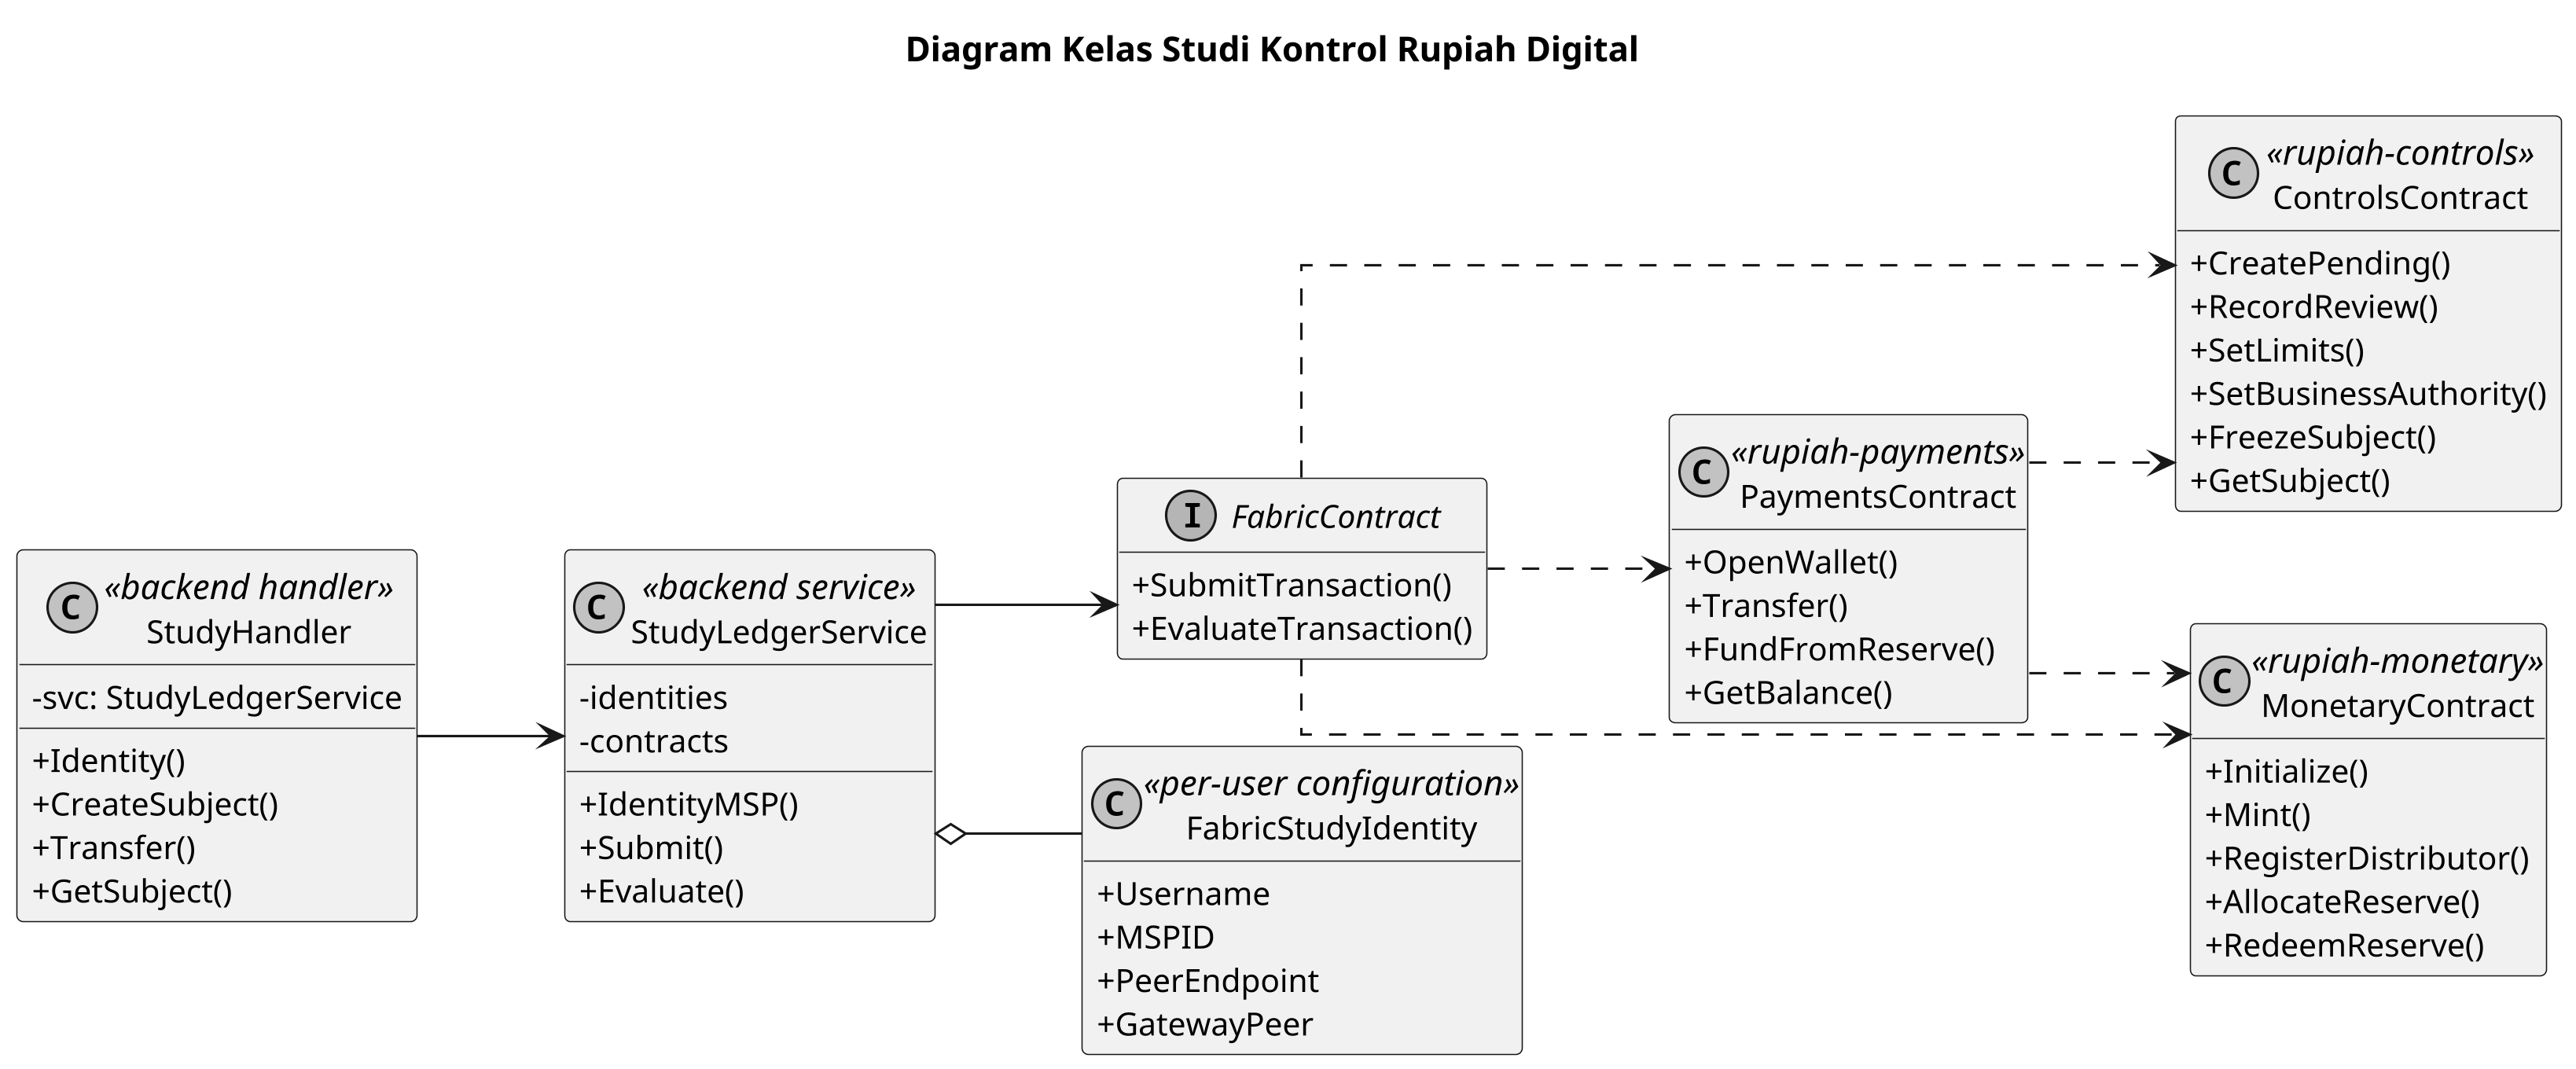
\includegraphics[width=\textwidth,height=0.78\textheight,keepaspectratio]{contents/chapter-3/controls-study-class.png}
  \caption{Diagram kelas layanan backend dan tiga \textit{chaincode} pada studi kontrol.}
  \label{fig:ch3-study-class}
\end{figure}

\begin{figure}[p]
  \centering
  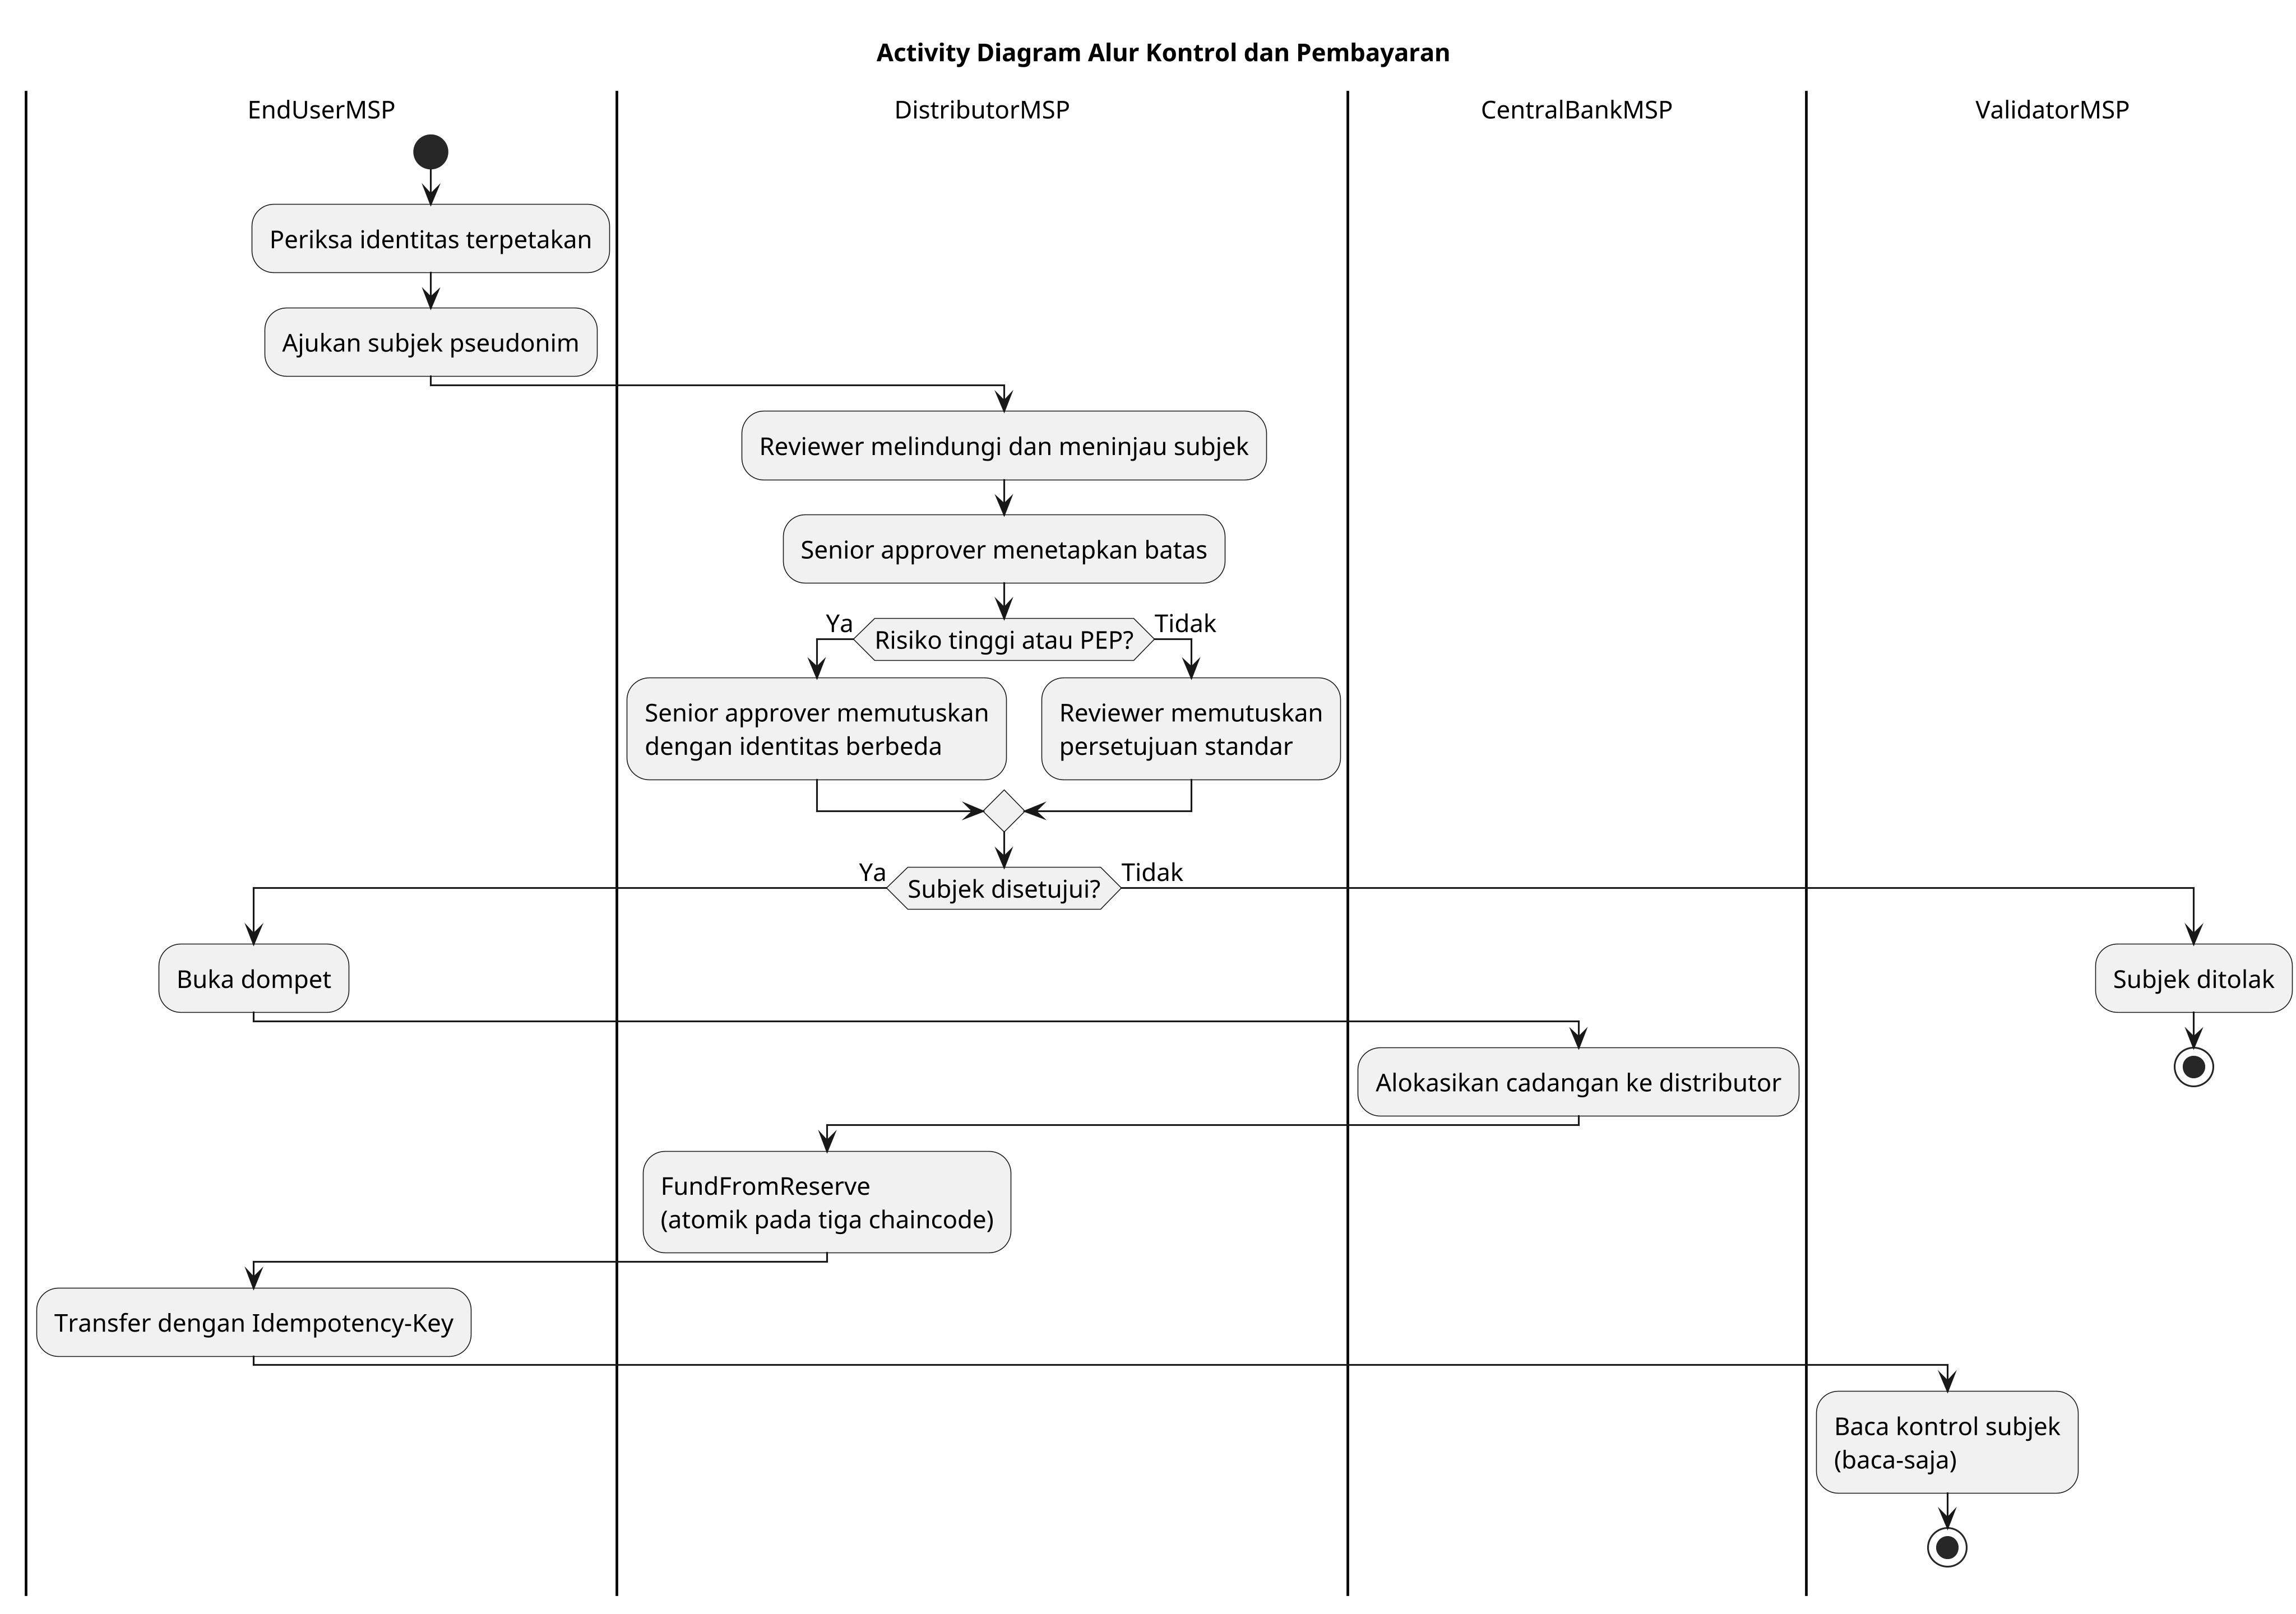
\includegraphics[width=\textwidth,height=0.78\textheight,keepaspectratio]{contents/chapter-3/controls-study-activity.png}
  \caption{Activity diagram alur onboarding subjek, persetujuan, pendanaan, dan transfer pada studi kontrol.}
  \label{fig:ch3-study-activity}
\end{figure}

\begin{figure}[p]
  \centering
  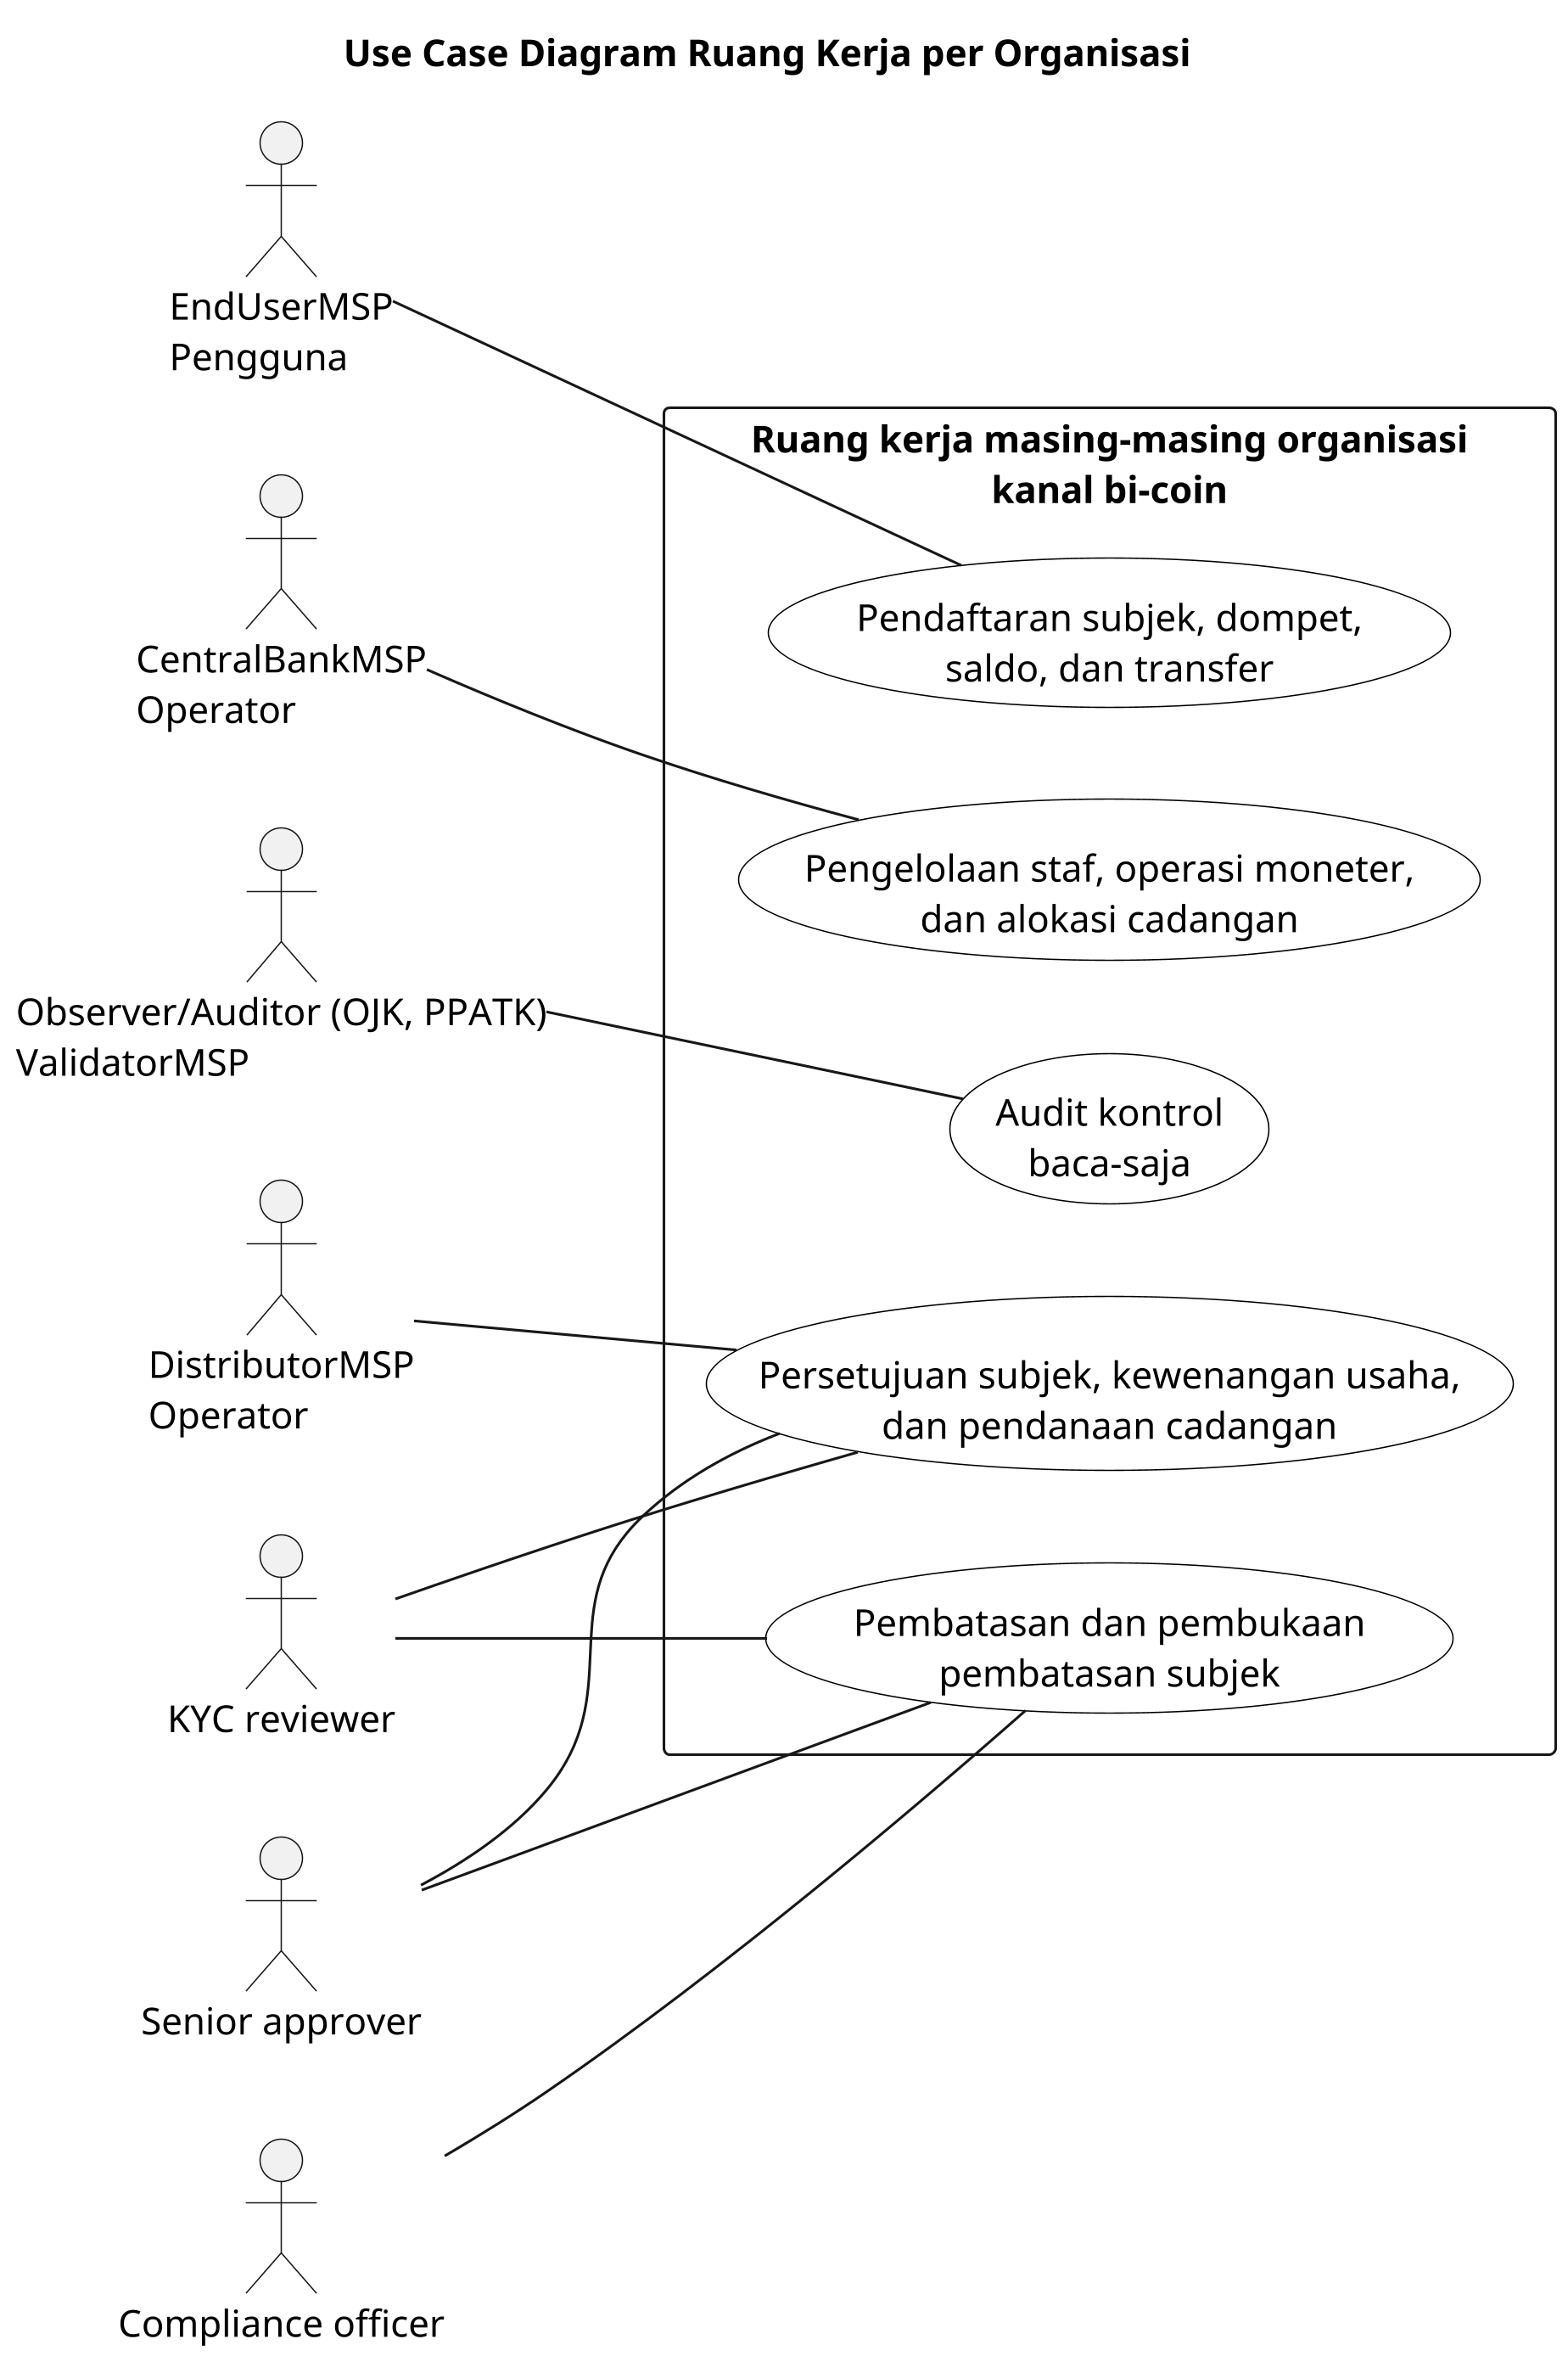
\includegraphics[width=\textwidth,height=0.78\textheight,keepaspectratio]{contents/chapter-3/controls-study-use-case.png}
  \caption{Diagram use case fungsi empat organisasi pada studi kontrol.}
  \label{fig:ch3-study-use-case}
\end{figure}

\begin{figure}[p]
  \centering
  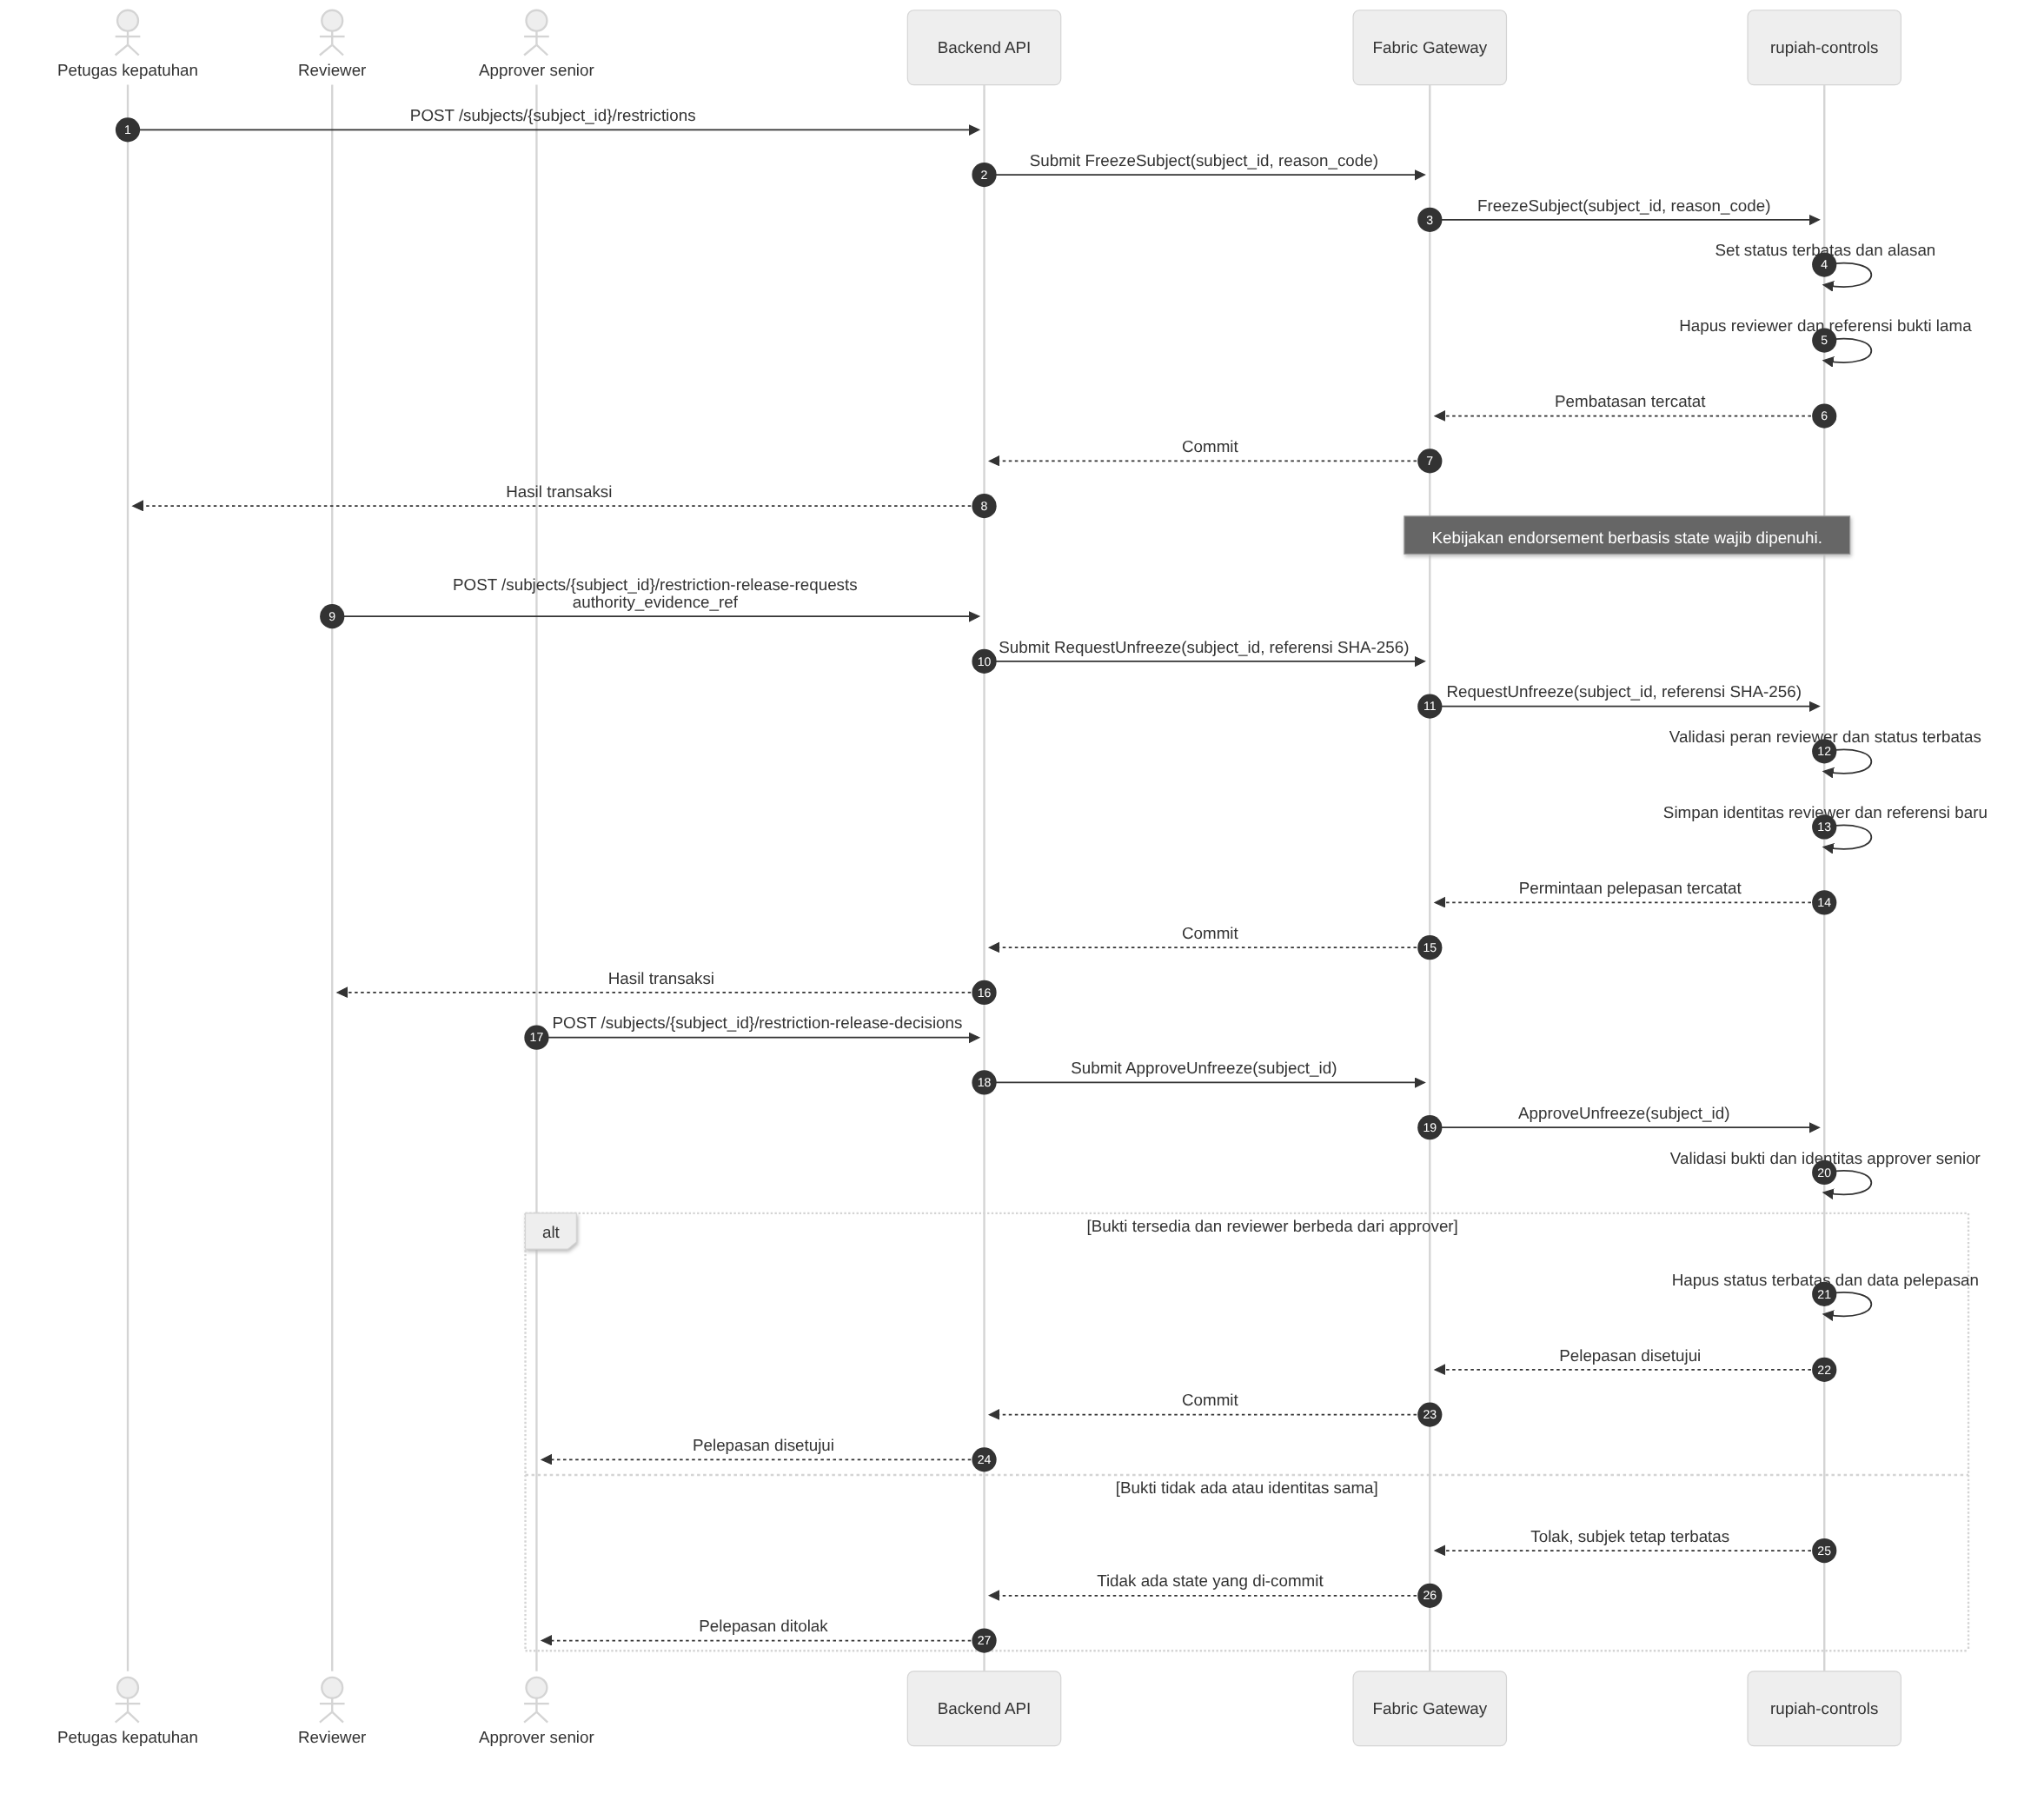
\includegraphics[width=\textwidth,height=0.78\textheight,keepaspectratio]{contents/chapter-3/controls-study-sequence-release.png}
  \caption{Urutan pembatasan subjek dan pelepasan pembatasan dengan bukti otoritas dan dua identitas staf berbeda.}
  \label{fig:ch3-study-sequence-release}
\end{figure}

\begin{figure}[p]
  \centering
  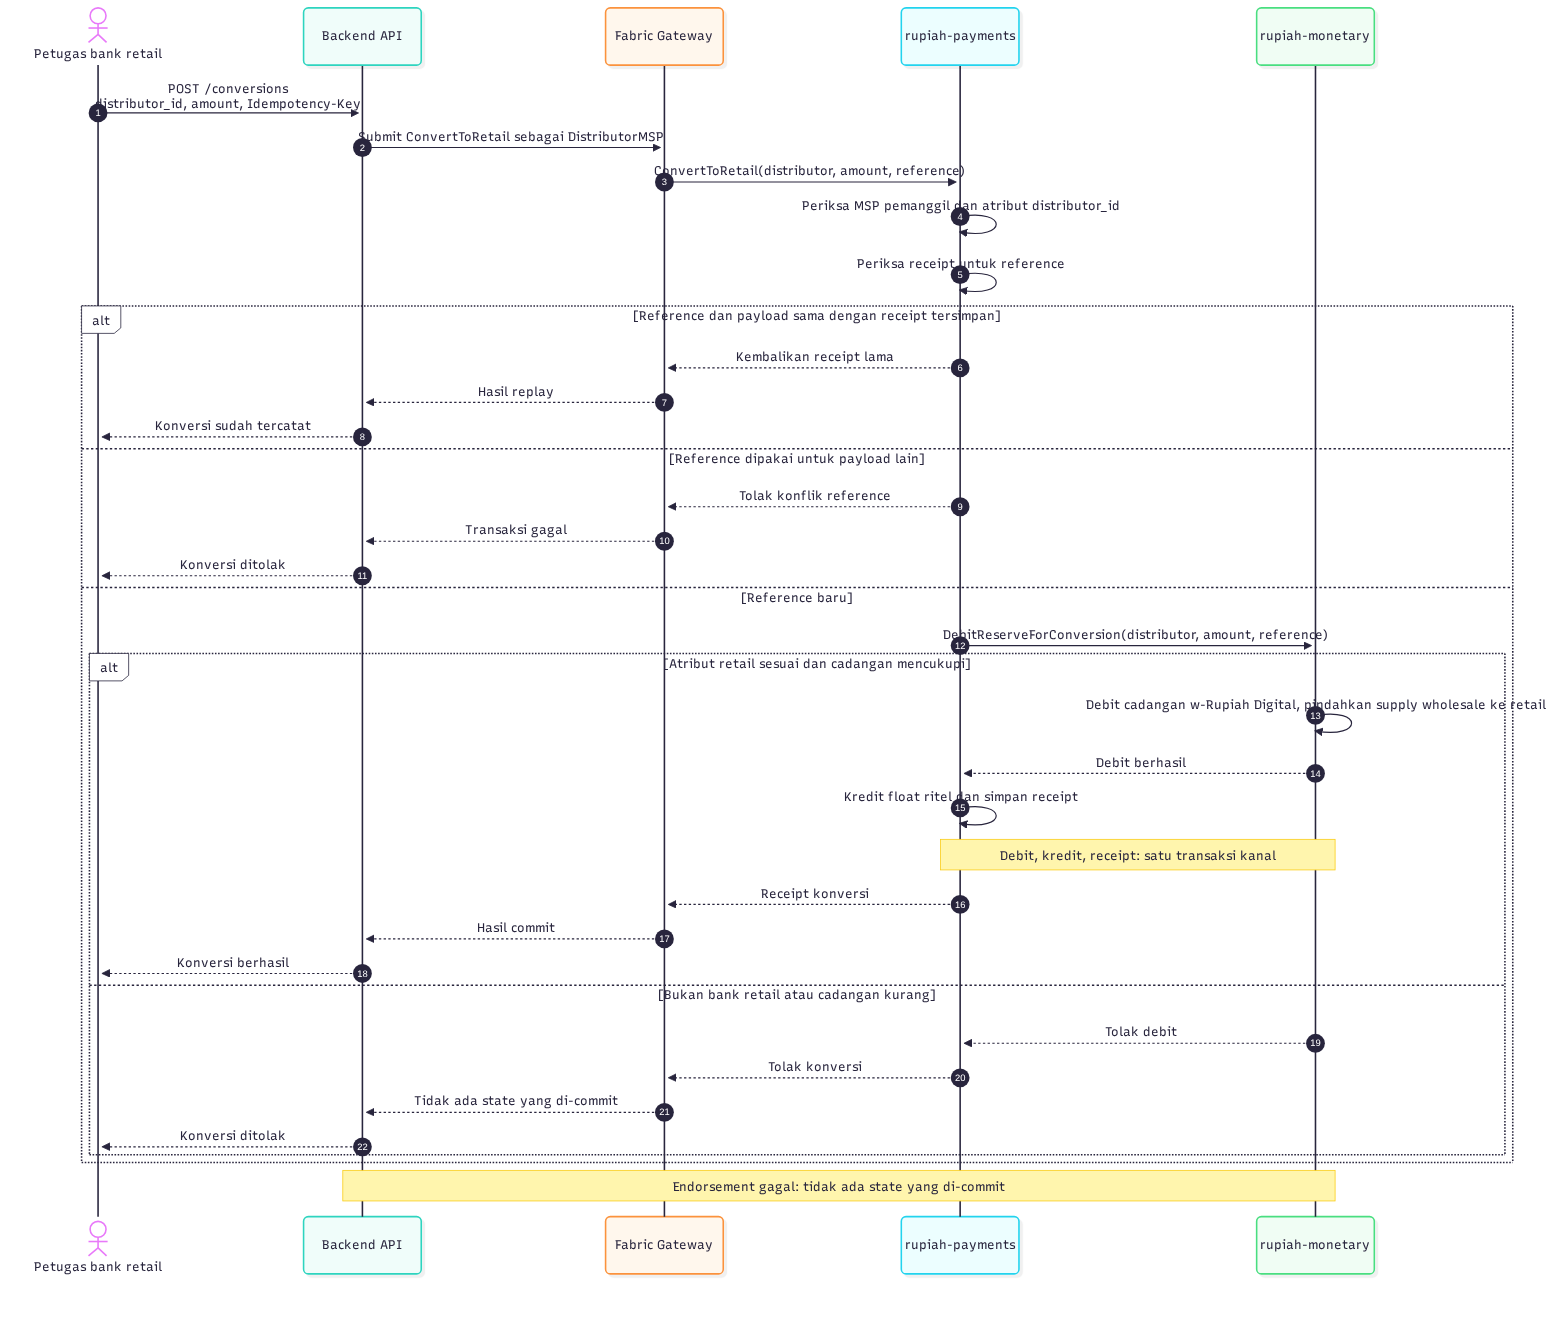
\includegraphics[width=\textwidth,height=0.78\textheight,keepaspectratio]{contents/chapter-3/controls-study-sequence-conversion.png}
  \caption{Urutan konversi cadangan \textit{w-Rupiah Digital} menjadi float \textit{r-Rupiah Digital} pada bank \textit{retail} dalam satu transaksi kanal.}
  \label{fig:ch3-study-sequence-conversion}
\end{figure}

\begin{figure}[p]
  \centering
  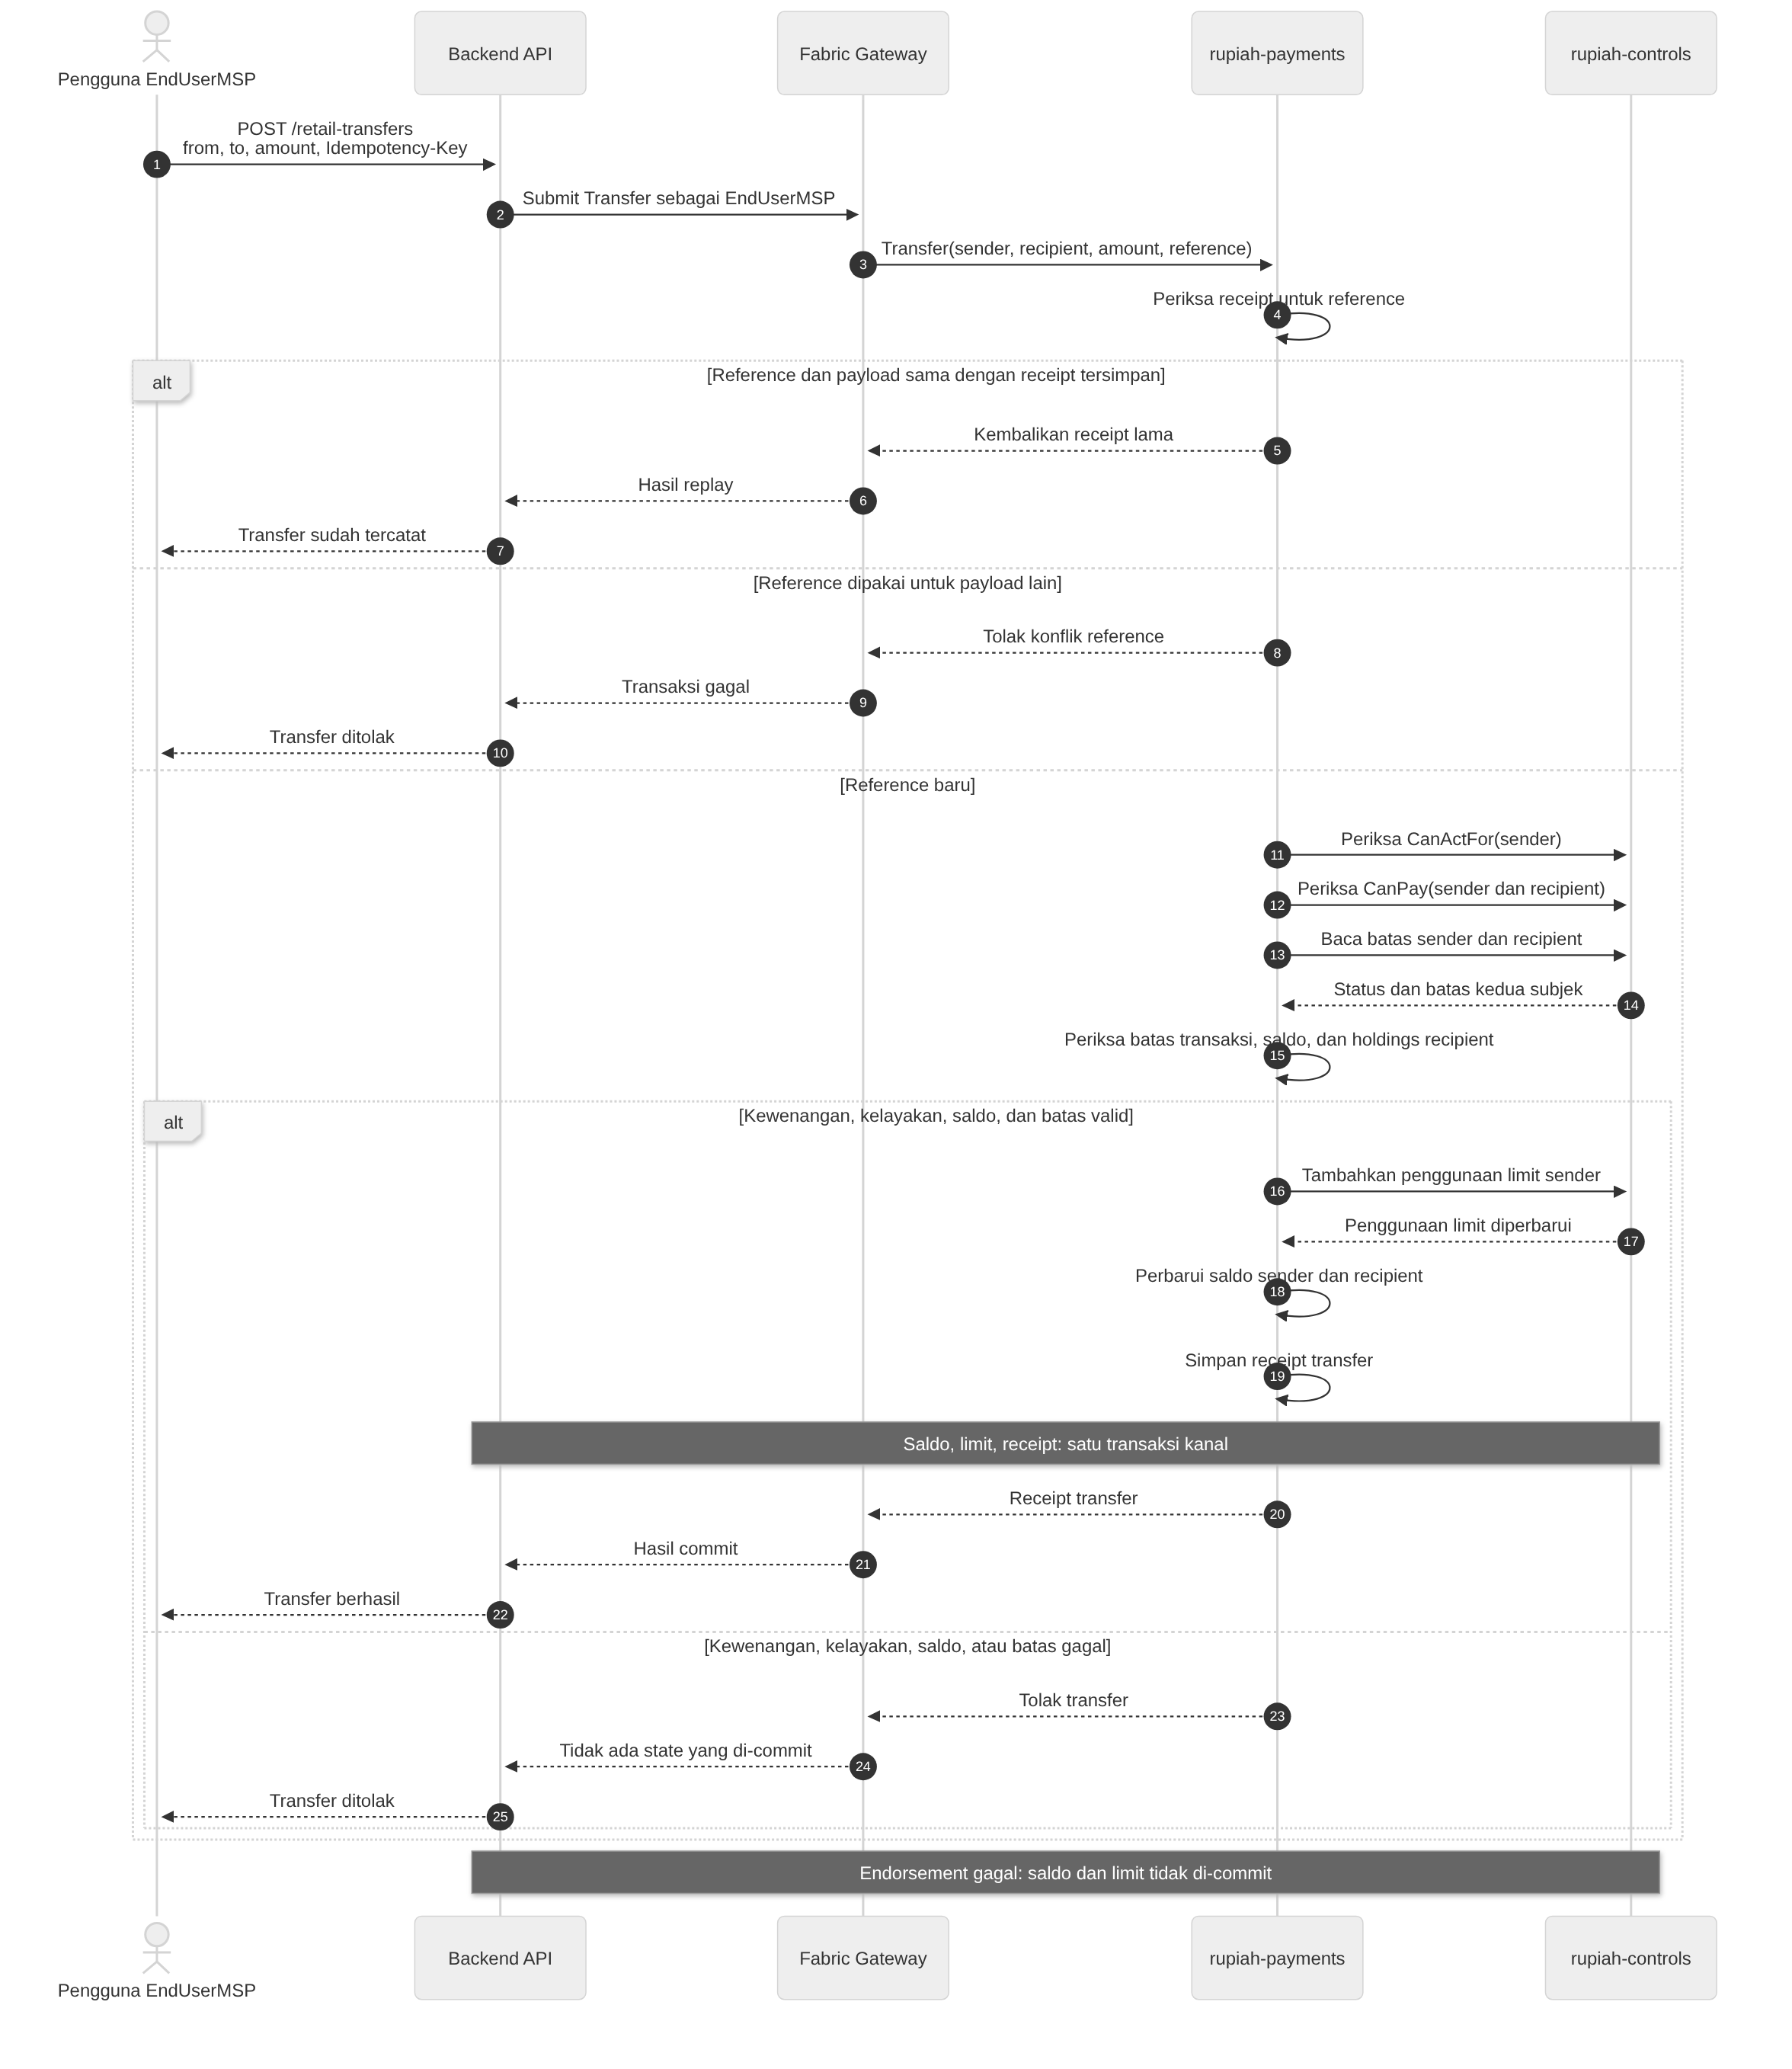
\includegraphics[width=\textwidth,height=0.78\textheight,keepaspectratio]{contents/chapter-3/controls-study-sequence-transfer.png}
  \caption{Urutan transfer ritel dengan pemeriksaan kewenangan, kelayakan, batas, saldo, dan receipt.}
  \label{fig:ch3-study-sequence-transfer}
\end{figure}

